\documentclass[11pt,reqno]{amsart}

\usepackage[utf8]{inputenc}
\usepackage[T1]{fontenc}
\usepackage{lmodern}
\usepackage{amsmath,amssymb,amsfonts,amsthm,mathtools}
\usepackage{booktabs,array,multirow}
\usepackage{graphicx}
\usepackage{enumitem}
\usepackage[margin=1.0in]{geometry}
\usepackage{microtype}
\usepackage{xcolor}
\definecolor{linkblue}{rgb}{0.0,0.2,0.6}
\usepackage[colorlinks=true,linkcolor=linkblue,citecolor=linkblue,urlcolor=linkblue]{hyperref}

\newtheorem{theorem}{Theorem}[section]
\newtheorem{proposition}[theorem]{Proposition}
\newtheorem{lemma}[theorem]{Lemma}
\newtheorem{corollary}[theorem]{Corollary}
\theoremstyle{definition}
\newtheorem{definition}[theorem]{Definition}
\theoremstyle{remark}
\newtheorem{remark}[theorem]{Remark}

\numberwithin{equation}{section}
\allowdisplaybreaks

\newcommand{\R}{\mathbb{R}}
\newcommand{\C}{\mathbb{C}}
\newcommand{\N}{\mathbb{N}}
\newcommand{\Z}{\mathbb{Z}}
\newcommand{\dd}{\mathrm{d}}
\newcommand{\ee}{\mathrm{e}}
\newcommand{\ii}{\mathrm{i}}
\newcommand{\Rea}{\mathrm{Re}}
\newcommand{\Ima}{\mathrm{Im}}
\newcommand{\PV}{\mathrm{P.V.}}
\newcommand{\sinch}{\mathrm{sinc}_{\mathrm{hyp}}}
\newcommand{\fac}{\mathclose{\mathchar"0021}}

\title[De Bruijn--Newman Velocity, Wigner Factorization, and Dipole PDE Hierarchy]{De Bruijn--Newman Heat-Flow Velocity $\left.\frac{\mathrm{d}\gamma_k}{\mathrm{d}\tau}\right|_{\tau=0} \equiv \frac{1}{4}\kappa(\gamma_k)$, Cross-Term-Free Gaussian Wigner Factorization, and the Transverse Dipole Evolution PDE Hierarchy for Riemann's $\Xi$-Function}

\author{Thijs Missiaen}
\address{Independent Researcher, Belgium}
\email{thijs.missiaen@gmail.com}
\thanks{ORCID: \href{https://orcid.org/0009-0007-3678-0810}{0009-0007-3678-0810}}

\subjclass[2020]{Primary 11M06, 11M26; Secondary 30D15, 35K05}
\keywords{Riemann $\Xi$-function, De~Bruijn--Newman constant, backwards heat equation, Chladni nodal curvature, Calogero--Moser Dyson system, Wigner phase-space factorization, pitchfork saddle coalescence, transverse Wronskian, dipole PDE hierarchy, Lehmer pairs}
\dedicatory{\upshape October 25, 2026}
\date{October 25, 2026}

\begin{document}
\sloppy

\begin{abstract}
We establish three exact analytical laws connecting the De~Bruijn--Newman heat-flow deformation $\Phi_\tau(u) := \Phi(u)\ee^{\tau u^2}$ and $\Xi_\tau(z) := 8\int_0^\infty \Phi(u)\ee^{\tau u^2}\cos(2zu)\,\dd u$ ($\partial_\tau\Xi_\tau \equiv -\frac{1}{4}\partial_z^2\Xi_\tau$, $\tau = 4t_{\mathrm{DBN}}$) to the transverse Chladni, Wigner, and dipole-cascade geometry of Riemann's $\Xi$-function. First, at $\tau = 0$ every simple zero $\gamma_k(\tau)$ moves with initial velocity $\left.\frac{\dd\gamma_k}{\dd\tau}\right|_{\tau=0} = \frac{\Xi''(\gamma_k)}{4\,\Xi'(\gamma_k)} \equiv \frac{1}{4}\kappa(\gamma_k) = \frac{1}{2}c_{\mathrm{par}}(\gamma_k)$ and every critical-line extremum $\tau_k(\tau)$ moves with velocity $\left.\frac{\dd\tau_k}{\dd\tau}\right|_{\tau=0} \equiv \frac{3}{4}\kappa_\Gamma(\tau_k)$, evaluating the principal-value Calogero--Moser sum in closed form as $\PV\sum_{\gamma_j\neq\gamma_k}(\gamma_k-\gamma_j)^{-1} \equiv \frac{1}{2}\kappa(\gamma_k)$. Second, in mirror coordinates $x = u+v, y = u-v$, the identity $u^2+v^2 \equiv \frac{1}{2}(x^2+y^2)$ yields the cross-term-free Gaussian Wigner factorization $G_{y,\tau}(x) \equiv \ee^{\frac{\tau}{2}y^2}\ee^{\frac{\tau}{2}x^2}G_y(x)$, preserving $|\Ima(x)| < \frac{\pi}{4}$ and shifting the pitchfork coalescence threshold with velocity $\left.\frac{\partial y_c}{\partial\tau}\right|_{\tau=0} = \frac{\eta_c}{\partial_y L_{y_c}'(\eta_c)} > 0$. Third, every transverse dipole invariant of $\widetilde{W}_\tau(d,t) = \sum_{m=1}^\infty c_{2m-1}(t;\tau)d^{2m-2}$ obeys the universal PDE hierarchy $\partial_\tau c_{2m-1} + \frac{1}{8}\partial_t^2 c_{2m-1} \equiv \frac{m(2m+1)}{4}c_{2m+1}$, governing Lehmer-pair backward coalescence via $\tau_{\mathrm{coal}}^{\mathrm{Lehmer}}(t_{\mathrm{mid}}) = -2\frac{c_1(t_{\mathrm{mid}};0)}{c_3(t_{\mathrm{mid}};0)}(1+\mathcal{O}(\delta^2)) < 0$.
\end{abstract}

\maketitle

\section{Introduction and Main Results}\label{sec:intro}

In the classical theory of the De~Bruijn--Newman constant $\Lambda$ initiated by P\'olya~\cite{polya1926}, De~Bruijn~\cite{debruijn1950}, and Newman~\cite{newman1976}, and developed quantitatively by Csordas, Norfolk, Smith, and Varga~\cite{csordas1986,csordas1988,csordas1994}, Rodgers and Tao~\cite{rodgerstao2020}, and the Polymath~15 project~\cite{polymath2019}, Riemann's completed zeta function $\Xi(z) := \xi(\frac{1}{2}+\ii z) = 8\int_0^\infty \Phi(u)\cos(2zu)\,\dd u$~\cite{riemann1859,titchmarsh1986} is embedded into a one-parameter family of entire functions of order one by multiplying the Jacobi--Riemann theta kernel $\Phi(u)$ by the Gaussian heat weight $\ee^{\tau u^2}$:
\begin{equation}\label{eq:intro_xi_tau}
\Phi_\tau(u) := \Phi(u)\,\ee^{\tau u^2}, \qquad \Xi_\tau(z) := 8\int_0^{\infty} \Phi(u)\,\ee^{\tau u^2}\cos(2zu)\,\dd u \qquad (z = t - \ii d \in \C,\; \tau \in \R).
\end{equation}
In our canonical logarithmic coordinate $u$ (related to the classical integration variable $w = 2u$ of~\cite{debruijn1950,newman1976,csordas1994,rodgerstao2020} by $\ee^{t_{\mathrm{DBN}}w^2} = \ee^{4t_{\mathrm{DBN}}u^2}$, so that $\tau = 4t_{\mathrm{DBN}}$ and the De~Bruijn--Newman threshold is $\tau_{\mathrm{DBN}} = 4\Lambda$), the deformed function $\Xi_\tau(z)$ satisfies the backwards heat-flow partial differential equation $\partial_\tau\Xi_\tau(z) = -\frac{1}{4}\partial_z^2\Xi_\tau(z)$. While the longitudinal dynamics of the zeros $\gamma_k(\tau)$ along the critical line $d = 0$ have been extensively studied via the infinite Calogero--Moser / Dyson particle system~\cite{csordas1994,rodgerstao2020,polymath2019} and Lehmer-pair lower bounds~\cite{lehmer1956,csordas1988}, three structural questions connecting the longitudinal heat flow $\tau$ to the two-dimensional transverse geometry of the critical strip $d = \sigma - \frac{1}{2} > 0$~\cite{speiser1934,hinkkanen1997,lagarias1999} have remained open:
\begin{enumerate}[label=\textup{(\arabic*)},leftmargin=2.2em]
\item \textit{Geometric duality between longitudinal heat-flow velocity and transverse Chladni nodal curvature.} When the real and imaginary nodal curves $R(d,t) = 0$ and $I(d,t) = 0$ of $\Xi(t - \ii d) = R(d,t) + \ii\,I(d,t)$ depart orthogonally from the critical line $d = 0$ into the strip $d > 0$ (Paper~III~\cite{missiaen2026paper3}), how are their static parabolic curvatures $\kappa(\gamma_k)$ and $\kappa_\Gamma(\tau_k)$ related to the dynamical De~Bruijn--Newman velocities $\gamma_k'(0)$ and $\tau_k'(0)$, and does this relation evaluate the conditionally convergent infinite Calogero--Moser sum in closed form?
\item \textit{Exact Wigner phase-space factorization under Gaussian deformation.} In the Wigner representation $W_\tau(d,t) = 8\int_0^\infty y\sinh(2dy)\,I_\tau(y,2t)\,\dd y$~\cite{wigner1932,hudson1974} (Paper~I~\cite{missiaen2026paper1}), does the Gaussian weight $\ee^{\tau(u^2+v^2)}$ introduce a mixed $xy$ cross-term in mirror coordinates $(x = u+v, y = u-v)$, or does it factor cleanly into an outer hyperbolic shift weight and an inner holomorphic contour kernel preserving the pitchfork saddle-point coalescence in $|\Ima(x)| < \frac{\pi}{4}$?
\item \textit{Exact evolution hierarchy for the transverse dipole invariants $c_{2m-1}(t;\tau)$.} In Papers~II and~IV~\cite{missiaen2026paper2,missiaen2026paper4}, the parity-reduced Wronskian $\widetilde{W}_\tau(d,t) := W_\tau(d,t)/d = \sum_{m=1}^\infty c_{2m-1}(t;\tau)d^{2m-2}$ was shown to obey a universal square-cascade at multiple zeros and Lehmer pairs. What is the exact partial differential equation governing the evolution of every dipole invariant $c_{2m-1}(t;\tau)$ under $\tau$?
\end{enumerate}

Building upon the frameworks established in Papers~I--X of this series~\cite{missiaen2026paper1,missiaen2026paper2,missiaen2026paper3,missiaen2026paper4,missiaen2026paper5,missiaen2026paper6,missiaen2026paper7,missiaen2026paper8,missiaen2026paper9,missiaen2026paper10}, the present work (Paper~XI) resolves these three questions through three exact analytical theorems.

\begin{theorem}[De Bruijn--Newman Chladni Velocity Duality, Cross-Term-Free Gaussian Wigner Factorization, and Universal Dipole PDE Hierarchy]\label{thm:main}
Let $z = t - \ii d \in \C$ and $\tau \in \R$, let $\Phi_\tau(u) := \Phi(u)\ee^{\tau u^2}$, and let $\Xi_\tau(z) := 8\int_0^\infty \Phi(u)\ee^{\tau u^2}\cos(2zu)\,\dd u = R_\tau(d,t) + \ii\,I_\tau(d,t)$ with parity-reduced transverse Wronskian $\widetilde{W}_\tau(d,t) := \frac{1}{2d}\partial_d|\Xi_\tau(t-\ii d)|^2 = \sum_{m=1}^\infty c_{2m-1}(t;\tau)d^{2m-2}$. Then the following three structural laws hold:
\begin{enumerate}[label=\textup{(\roman*)},leftmargin=2.2em]
\item \textbf{Backwards Heat-Flow PDE, Parabolic Chladni Curvature Duality, and Closed-Form Dyson Sum.} The function $\Xi_\tau(z)$ satisfies $\partial_\tau\Xi_\tau(z) \equiv -\frac{1}{4}\partial_z^2\Xi_\tau(z)$ on $\C\times\R$. At $\tau = 0$, every simple real zero $\gamma_k(\tau)$ ($\Xi(\gamma_k) = 0, \Xi'(\gamma_k) \neq 0$) and every non-degenerate critical-line extremum $\tau_k(\tau)$ ($\Xi'(\tau_k) = 0, \Xi''(\tau_k) \neq 0$) move with exact initial velocities
\begin{equation}\label{eq:intro_velocity_duality}
\left.\frac{\dd\gamma_k}{\dd\tau}\right|_{\tau=0} = \frac{\Xi''(\gamma_k)}{4\,\Xi'(\gamma_k)} \equiv \frac{1}{4}\kappa(\gamma_k) = \frac{1}{2}c_{\mathrm{par}}(\gamma_k), \qquad \left.\frac{\dd\tau_k}{\dd\tau}\right|_{\tau=0} = \frac{\Xi'''(\tau_k)}{4\,\Xi''(\tau_k)} \equiv \frac{3}{4}\kappa_\Gamma(\tau_k),
\end{equation}
where $\kappa(\gamma_k) := t_{\mathcal{R}_k}''(0)$ and $\kappa_\Gamma(\tau_k) := \tau_{\Gamma_k}''(0)$ are the parabolic Chladni curvatures of $R(d,t) = 0$ and $I(d,t) = 0$ at $d = 0$, and the principal-value Calogero--Moser / Dyson interaction sum is evaluated in closed form by
\begin{equation}\label{eq:intro_dyson_closed}
\begin{aligned}
\PV\sum_{\gamma_j \neq \gamma_k} \frac{1}{\gamma_k - \gamma_j} &:= \frac{1}{2\gamma_k} + \sum_{\substack{m=1 \\ m \neq k}}^{\infty} \frac{2\gamma_k}{\gamma_k^2 - \gamma_m^2} \\
&\equiv \frac{\Xi''(\gamma_k)}{2\,\Xi'(\gamma_k)} = \frac{1}{2}\kappa(\gamma_k) = -\frac{1}{2}\Ima\!\left(2g_1\!\left(\tfrac{1}{2}+\ii\gamma_k\right) + \frac{\zeta''(\frac{1}{2}+\ii\gamma_k)}{\zeta'(\frac{1}{2}+\ii\gamma_k)}\right).
\end{aligned}
\end{equation}
\item \textbf{Cross-Term-Free Gaussian Wigner Factorization and Pitchfork Coalescence Shift.} In mirror coordinates $x = u+v$ and $y = u-v$, the identity $u^2+v^2 \equiv \frac{1}{2}(x^2+y^2)$ yields the cross-term-free factorization $G_{y,\tau}(x) := \Phi_\tau(\frac{x+y}{2})\Phi_\tau(\frac{x-y}{2}) \equiv \ee^{\frac{\tau}{2}y^2}\ee^{\frac{\tau}{2}x^2}G_y(x)$ and Wigner correlation PDE $\partial_\tau I_\tau(y,\omega) \equiv \frac{1}{2}(y^2 - \partial_\omega^2)I_\tau(y,\omega) \equiv \frac{1}{8}((2y)^2 - \partial_t^2)I_\tau(y,2t)$ ($\omega = 2t$), preserving the holomorphic strip $|\Ima(x)| < \frac{\pi}{4}$ for all $\tau \in \R$ and shifting the pitchfork coalescence threshold $y_c(\omega;\tau)$ with strictly positive initial velocity
\begin{equation}\label{eq:intro_yc_shift}
\left.\frac{\partial y_c(\omega;\tau)}{\partial\tau}\right|_{\tau=0} = \frac{\eta_c(\omega;0)}{\partial_y L_{y_c}'\bigl(\eta_c(\omega;0)\bigr)} > 0.
\end{equation}
\item \textbf{Universal Transverse Dipole Evolution PDE Hierarchy and Lehmer Coalescence Law.} The parity-reduced Wronskian $\widetilde{W}_\tau(d,t)$ satisfies the fourth-order radial wave-heat PDE $\partial_\tau\widetilde{W}_\tau + \frac{1}{8}(\partial_t^2 - \partial_d^2 - \frac{2}{d}\partial_d)\widetilde{W}_\tau \equiv 0$ together with $\partial_\tau\widetilde{W}_\tau + \frac{1}{4}\partial_t^2\widetilde{W}_\tau \equiv \frac{1}{8}(\partial_t^2 + \partial_d^2 + \frac{2}{d}\partial_d)\widetilde{W}_\tau \equiv \frac{1}{2}\widetilde{W}_{1,2;\tau}(d,t)$ ($\widetilde{W}_{1,2;\tau} := \frac{1}{2d}\partial_d|\Xi_\tau'(t-\ii d)|^2$), and every transverse dipole invariant $c_{2m-1}(t;\tau)$ obeys the universal PDE hierarchy
\begin{equation}\label{eq:intro_dipole_pde}
\frac{\partial c_{2m-1}}{\partial\tau}(t;\tau) + \frac{1}{8}\,\frac{\partial^2 c_{2m-1}}{\partial t^2}(t;\tau) \equiv \frac{m(2m+1)}{4}\,c_{2m+1}(t;\tau) \qquad (\forall\, m \ge 1).
\end{equation}
At any $m$-fold coalescence point $t_0$ ($m \ge 2$), $\partial_\tau c_{2m-3}(t_0;\tau_{\mathrm{coal}}) \equiv \frac{m}{4}c_{2m-1}(t_0;\tau_{\mathrm{coal}}) = \frac{m^2}{4(m\fac)^2}(\partial_t^m\Xi_{\tau_{\mathrm{coal}}}(t_0))^2 > 0$, and across any closely spaced Lehmer pair $t_\pm = t_{\mathrm{mid}} \pm \delta$ ($\delta > 0$), $\left.\frac{\partial c_1}{\partial\tau}\right|_{(t_{\mathrm{mid}},0)} \equiv \frac{1}{4}(\Xi''(t_{\mathrm{mid}}))^2 + \frac{1}{4}\Xi(t_{\mathrm{mid}})\Xi^{(4)}(t_{\mathrm{mid}}) > 0$, recovering the backward coalescence threshold $\tau_{\mathrm{coal}}^{\mathrm{Lehmer}}(t_{\mathrm{mid}}) = -2\frac{c_1(t_{\mathrm{mid}};0)}{c_3(t_{\mathrm{mid}};0)}(1 + \mathcal{O}(\delta^2)) = -2\delta^2(1 + \mathcal{O}(\delta^2)) < 0$.
\end{enumerate}
\end{theorem}

The canonical quantitative constants governing Theorem~\ref{thm:main} are given explicitly by
\begin{equation}\label{eq:canonical_constants}
\begin{aligned}
\kappa(\gamma_1) &= -1.1592611550\dots, & \left.\frac{\dd\gamma_1}{\dd\tau}\right|_{\tau=0} &= \frac{1}{4}\kappa(\gamma_1) = -0.2898152887\dots, \\
\left.\frac{\dd(\gamma_{10}-\gamma_9)}{\dd\tau}\right|_{\tau=0} &= +0.3866151652\dots > 0, & \left.\frac{\partial y_c(2\gamma_1;\tau)}{\partial\tau}\right|_{\tau=0} &= +0.0125362327\dots > 0, \\
\tau_{\mathrm{coal}}^{\mathrm{Lehmer}}(\gamma_9,\gamma_{10}) &= -1.34840873\dots, & \tau_{\mathrm{coal}}^{\mathrm{Lehmer}}(\gamma_{6709},\gamma_{6710}) &= -7.096664 \times 10^{-4}.
\end{aligned}
\end{equation}

\subsection{Proof overview}\label{subsec:proof_overview}

The proof of Theorem~\ref{thm:main} combines three quantitative ingredients developed in Sections~\ref{sec:chladni_velocity}--\ref{sec:dipole_hierarchy}:
\begin{enumerate}[label=\textup{(\arabic*)},leftmargin=2.2em]
\item \textit{Harmonic Cauchy--Riemann curvature versus backwards heat-flow differentiation (Section~\ref{sec:chladni_velocity}).} Because $\Phi(u) \ll \ee^{9|u|}\exp(-\pi\ee^{4|u|})$ decays double-exponentially, differentiating $\Xi_\tau(z)$ under the integral sign yields $\partial_\tau\Xi_\tau = -\frac{1}{4}\partial_z^2\Xi_\tau$. Since the two-dimensional Laplace equation $\partial_d^2 R = -\partial_t^2 R$ on the critical line $d = 0$ and the one-dimensional backwards heat equation $\partial_\tau\Xi_\tau = -\frac{1}{4}\partial_t^2\Xi_\tau$ at $\tau = 0$ are governed by the identical operator $-\partial_t^2$, implicit differentiation of $\Xi_\tau(\gamma_k(\tau)) = 0$ and $\partial_t\Xi_\tau(\tau_k(\tau)) = 0$ directly identifies $\gamma_k'(0)$ and $\tau_k'(0)$ with the Chladni curvatures $\frac{1}{4}\kappa(\gamma_k)$ and $\frac{3}{4}\kappa_\Gamma(\tau_k)$, while matching the regular part of $\Xi'(z)/\Xi(z)$ at $z = \gamma_k$ evaluates the Calogero--Moser sum~\eqref{eq:intro_dyson_closed}.
\item \textit{Parallelogram diagonalization in mirror coordinates and implicit pitchfork perturbation (Section~\ref{sec:wigner_factorization}).} Under the orthogonal rotation $u = \frac{x+y}{2}, v = \frac{x-y}{2}$, the quadratic form $u^2 + v^2 = \frac{1}{2}(x^2 + y^2)$ is diagonal. Consequently, $G_{y,\tau}(x) = \ee^{\frac{\tau}{2}y^2}\ee^{\frac{\tau}{2}x^2}G_y(x)$ factors without an $xy$ cross-term, preserving the double-exponential closure of the Cauchy contour box in $|\Ima(x)| < \frac{\pi}{4}$. Differentiating the simultaneous pitchfork bifurcation system $L_{y_c}'(\eta_c) - \tau\eta_c = \omega$ and $L_{y_c}''(\eta_c) = \tau$ at $\tau = 0$, the term $L_{y_c}''(\eta_c)\,\partial_\tau\eta_c$ vanishes identically by the coalescence condition $L_{y_c}''(\eta_c) = 0$, isolating~\eqref{eq:intro_yc_shift}.
\item \textit{Radial wave-heat operator cancellation and Taylor moment hierarchy (Section~\ref{sec:dipole_hierarchy}).} For $M_\tau(d,t) := |\Xi_\tau(t-\ii d)|^2$, the gradient squares $+2|\Xi_\tau'|^2$ in $\partial_t^2 M_\tau$ and $\partial_d^2 M_\tau$ cancel identically in $(\partial_t^2 - \partial_d^2)M_\tau = -8\,\partial_\tau M_\tau$ and add in $(\partial_t^2 + \partial_d^2)M_\tau = 4|\Xi_\tau'|^2$. Applying $\frac{1}{2d}\partial_d$ and expanding $\widetilde{W}_\tau(d,t) = \sum_{m=1}^\infty c_{2m-1}(t;\tau)d^{2m-2}$ yields the coupled hierarchy~\eqref{eq:intro_dipole_pde}, which we combine with the Weierstrass normal form at Lehmer pairs to establish the backward coalescence law.
\end{enumerate}

\subsection{Notation and conventions}\label{subsec:notation}

Throughout this paper, $s = \sigma + \ii t = \frac{1}{2} + d + \ii t$ with $d = \sigma - \frac{1}{2} \in \R$ and $z = -\ii(s - \frac{1}{2}) = t - \ii d$. Riemann's completed zeta function is $\xi(s) := \frac{1}{2}s(s-1)\pi^{-s/2}\Gamma(\frac{s}{2})\zeta(s) = G(s)\zeta(s)$, where $G(s) := \frac{1}{2}s(s-1)\pi^{-s/2}\Gamma(\frac{s}{2})$ has logarithmic derivative $g_1(s) := \frac{G'(s)}{G(s)} = \frac{1}{s} + \frac{1}{s-1} - \frac{1}{2}\ln\pi + \frac{1}{2}\psi(\frac{s}{2})$. For $\tau \in \R$, the De~Bruijn--Newman deformed function is $\Xi_\tau(z) := 8\int_0^\infty \Phi(u)\ee^{\tau u^2}\cos(2zu)\,\dd u = R_\tau(d,t) + \ii\,I_\tau(d,t)$, where $\Phi(u) := \sum_{m=1}^\infty (2\pi^2 m^4\ee^{9u} - 3\pi m^2\ee^{5u})\exp(-\pi m^2\ee^{4u})$ satisfies $\Phi(-u) = \Phi(u) > 0$. The transverse Wronskian is $W_\tau(d,t) := \frac{1}{2}\partial_d|\Xi_\tau(t-\ii d)|^2 = R_\tau\,\partial_d R_\tau + I_\tau\,\partial_d I_\tau = \Ima(\overline{\Xi_\tau(t-\ii d)}\,\partial_z\Xi_\tau(t-\ii d))$, and the parity-reduced Wronskian is $\widetilde{W}_\tau(d,t) := W_\tau(d,t)/d$. All numerical values are computed at $60$-decimal working precision (\texttt{mpmath.mp.dps = 60}) and certified via $35$-decimal directed-rounding interval arithmetic (\texttt{mpmath.iv.dps = 35}) in \texttt{scripts/}\allowbreak\texttt{verify\_paper11\_}\allowbreak\texttt{debruijn\_newman\_}\allowbreak\texttt{chladni.py}.

\section{Backwards Heat-Flow PDE, Parabolic Chladni Zero-Curve Curvature \texorpdfstring{$\kappa(\gamma_k)$}{kappa(gamma\_k)}, and Closed-Form Calogero--Moser Sum}\label{sec:chladni_velocity}

Before differentiating $\Xi_\tau(z)$ with respect to $\tau$ and $z$, we establish the absolute and locally uniform convergence of all integral derivatives across $\C \times \R$. For real $u \ge 0$, the Jacobi--Riemann kernel satisfies $0 < \Phi(u) \le C_0\,\ee^{9u}\exp(-\pi\ee^{4u})$ with $C_0 = 2\pi^2\sum_{m=1}^\infty m^4\ee^{-\pi(m^2-1)} < 20$. For any bounded subset $K \subset \C \times \R$ with $|z| \le R$ and $|\tau| \le T$, and for any integers $j, k \ge 0$, the differentiated integrand satisfies
\begin{equation}\label{eq:premove_heat_bound}
\Bigl|\partial_\tau^j \partial_z^k\bigl[\Phi(u)\,\ee^{\tau u^2}\cos(2zu)\bigr]\Bigr| \le C_0\,(2u)^{2j+k}\exp\!\bigl(9u + Tu^2 + 2Ru - \pi\ee^{4u}\bigr) \qquad (u \ge 0).
\end{equation}
Because $\pi\ee^{4u}$ grows exponentially while $Tu^2 + (2R+9)u$ grows only quadratically, the right-hand side of~\eqref{eq:premove_heat_bound} is integrable on $[0, \infty)$ uniformly on $K$. By Lebesgue's dominated convergence theorem and Morera's theorem, $\Xi_\tau(z)$ is an even entire function of $z$ for every $\tau \in \R$ and is real-analytic in $(z, \tau) \in \C \times \R$, permitting termwise differentiation under the integral sign to all orders.

\begin{theorem}[Backwards Heat-Flow PDE and Parabolic Chladni Curvature Duality]\label{thm:chladni_velocity}
Let $\Phi_\tau(u) := \Phi(u)\ee^{\tau u^2}$ and $\Xi_\tau(z) := 8\int_0^\infty \Phi(u)\ee^{\tau u^2}\cos(2zu)\,\dd u$. Then:
\begin{enumerate}[label=\textup{(\roman*)},leftmargin=2.2em]
\item \textbf{Exact Backwards Heat-Flow PDE.} For all $(z, \tau) \in \C \times \R$, $\Xi_\tau(z)$ satisfies the backwards heat equation
\begin{equation}\label{eq:backwards_heat_pde}
\frac{\partial \Xi_\tau}{\partial\tau}(z) \equiv -\frac{1}{4}\,\frac{\partial^2 \Xi_\tau}{\partial z^2}(z) \qquad \left(\text{equivalently } \frac{\partial \Xi_\tau}{\partial t_{\mathrm{DBN}}}(z) \equiv -\frac{\partial^2 \Xi_\tau}{\partial z^2}(z) \text{ for } t_{\mathrm{DBN}} = \frac{\tau}{4}\right).
\end{equation}
\item \textbf{Initial Zero Velocity and Parabolic Chladni Zero-Curve Curvature $\kappa(\gamma_k)$.} Let $\gamma_k(\tau)$ be a simple zero of $\Xi_\tau$ continuing the $k$-th simple critical-line zero $\gamma_k = \gamma_k(0)$ of $\Xi(t)$, and let $\mathcal{R}_k : R(d, t_{\mathcal{R}_k}(d)) \equiv 0$ be the real Chladni nodal curve departing orthogonally into the critical strip $d > 0$ with Taylor expansion $t_{\mathcal{R}_k}(d) = \gamma_k + c_{\mathrm{par}}(\gamma_k)d^2 + c_{\mathrm{quart}}(\gamma_k)d^4 + \mathcal{O}(d^6)$ and parabolic curvature $\kappa(\gamma_k) := t_{\mathcal{R}_k}''(0) = 2c_{\mathrm{par}}(\gamma_k) = \frac{\Xi''(\gamma_k)}{\Xi'(\gamma_k)}$. Then for every $\tau$ where $\partial_z\Xi_\tau(\gamma_k(\tau)) \neq 0$, $\gamma_k'(\tau) = \frac{\partial_z^2\Xi_\tau(\gamma_k(\tau))}{4\,\partial_z\Xi_\tau(\gamma_k(\tau))}$, and at $\tau = 0$:
\begin{equation}\label{eq:gamma_velocity_duality}
\left.\frac{\dd\gamma_k}{\dd\tau}\right|_{\tau=0} = \frac{\Xi''(\gamma_k)}{4\,\Xi'(\gamma_k)} \equiv \frac{1}{4}\kappa(\gamma_k) \equiv \frac{1}{2}c_{\mathrm{par}}(\gamma_k) \equiv -\frac{1}{4}\Ima\!\left(2g_1\!\left(\tfrac{1}{2}+\ii\gamma_k\right) + \frac{\zeta''(\frac{1}{2}+\ii\gamma_k)}{\zeta'(\frac{1}{2}+\ii\gamma_k)}\right),
\end{equation}
while the second-order heat-flow acceleration at $\tau = 0$ is connected to the quartic Chladni coefficient $c_{\mathrm{quart}}(\gamma_k) = \frac{\Xi'''(\gamma_k)\kappa(\gamma_k)}{4\,\Xi'(\gamma_k)} - \frac{\Xi^{(4)}(\gamma_k)}{24\,\Xi'(\gamma_k)} - \frac{1}{8}\kappa(\gamma_k)^3$ by
\begin{equation}\label{eq:gamma_acceleration_duality}
\left.\frac{\dd^2\gamma_k}{\dd\tau^2}\right|_{\tau=0} = \frac{\Xi'''(\gamma_k)\,\kappa(\gamma_k)}{8\,\Xi'(\gamma_k)} - \frac{\Xi^{(4)}(\gamma_k)}{16\,\Xi'(\gamma_k)} - \frac{1}{16}\kappa(\gamma_k)^3 \equiv \frac{3}{2}c_{\mathrm{quart}}(\gamma_k) - \frac{\Xi'''(\gamma_k)\,\kappa(\gamma_k)}{4\,\Xi'(\gamma_k)} + \frac{1}{8}\kappa(\gamma_k)^3.
\end{equation}
\item \textbf{Initial Extremum Velocity and Imaginary Chladni Wall Curvature $\kappa_\Gamma(\tau_k)$.} Let $\tau_k(\tau) \in (\gamma_k(\tau), \gamma_{k+1}(\tau))$ be a non-degenerate critical-line extremum satisfying $\partial_t\Xi_\tau(\tau_k(\tau)) = 0$ and $\partial_t^2\Xi_\tau(\tau_k(\tau)) \neq 0$, and let $\Gamma_k : I(d, \tau_{\Gamma_k}(d)) \equiv 0$ be the imaginary Chladni chamber wall at $\tau = 0$ with parabolic wall curvature $\kappa_\Gamma(\tau_k) := \tau_{\Gamma_k}''(0) = \frac{\Xi'''(\tau_k)}{3\,\Xi''(\tau_k)}$. Then at $\tau = 0$:
\begin{equation}\label{eq:extremum_velocity_duality}
\left.\frac{\dd\tau_k}{\dd\tau}\right|_{\tau=0} = \frac{\Xi'''(\tau_k)}{4\,\Xi''(\tau_k)} \equiv \frac{3}{4}\kappa_\Gamma(\tau_k).
\end{equation}
\end{enumerate}
\end{theorem}

\begin{proof}
(i) Differentiating~\eqref{eq:intro_xi_tau} under the integral sign via~\eqref{eq:premove_heat_bound} gives $\partial_\tau\Xi_\tau(z) = 8\int_0^\infty u^2\Phi(u)\ee^{\tau u^2}\cos(2zu)\,\dd u$ and $\partial_z^2\Xi_\tau(z) = 8\int_0^\infty (-4u^2)\Phi(u)\ee^{\tau u^2}\cos(2zu)\,\dd u = -4\,\partial_\tau\Xi_\tau(z)$, proving~\eqref{eq:backwards_heat_pde}.

(ii) Since $\Xi_\tau(\gamma_k(\tau)) \equiv 0$ and $\partial_z\Xi_\tau(\gamma_k(\tau)) \neq 0$, the implicit function theorem guarantees that $\tau \mapsto \gamma_k(\tau)$ is real-analytic near $\tau = 0$, and differentiating $\Xi_\tau(\gamma_k(\tau)) = 0$ with respect to $\tau$ yields $\partial_\tau\Xi_\tau(\gamma_k(\tau)) + \partial_z\Xi_\tau(\gamma_k(\tau))\,\gamma_k'(\tau) = 0$. Substituting $\partial_\tau\Xi_\tau = -\frac{1}{4}\partial_z^2\Xi_\tau$ gives $\gamma_k'(\tau) = \frac{\partial_z^2\Xi_\tau(\gamma_k(\tau))}{4\,\partial_z\Xi_\tau(\gamma_k(\tau))}$. Meanwhile, on the critical strip $z = t - \ii d$ at $\tau = 0$, expanding $R(d,t) = \Rea\,\Xi(t-\ii d) = \Xi(t) - \frac{d^2}{2}\Xi''(t) + \frac{d^4}{24}\Xi^{(4)}(t) + \mathcal{O}(d^6)$ along the real nodal curve $t_{\mathcal{R}_k}(d) = \gamma_k + c_{\mathrm{par}}d^2 + c_{\mathrm{quart}}d^4 + \mathcal{O}(d^6)$ where $\Xi(\gamma_k) = 0$ gives, at order $d^2$, $\Xi'(\gamma_k)c_{\mathrm{par}} - \frac{1}{2}\Xi''(\gamma_k) = 0$, so $\kappa(\gamma_k) = t_{\mathcal{R}_k}''(0) = 2c_{\mathrm{par}}(\gamma_k) = \frac{\Xi''(\gamma_k)}{\Xi'(\gamma_k)}$, establishing the first three equalities in~\eqref{eq:gamma_velocity_duality}. Next, writing $\Xi(z) = G(s)\zeta(s)$ with $s = \frac{1}{2} + \ii z$ ($\frac{\dd s}{\dd z} = \ii$) and $G'(s) = g_1(s)G(s)$, the chain rule gives $\Xi'(z) = \ii(G'(s)\zeta(s) + G(s)\zeta'(s))$ and $\Xi''(z) = -(G''(s)\zeta(s) + 2G'(s)\zeta'(s) + G(s)\zeta''(s))$. Evaluating at $z = \gamma_k$ where $\zeta(s_k) = 0$ ($s_k = \frac{1}{2}+\ii\gamma_k$) yields
\[
\frac{\Xi''(\gamma_k)}{\Xi'(\gamma_k)} = -\frac{2G'(s_k)\zeta'(s_k) + G(s_k)\zeta''(s_k)}{\ii\,G(s_k)\zeta'(s_k)} = \ii\!\left(2g_1(s_k) + \frac{\zeta''(s_k)}{\zeta'(s_k)}\right) = -\Ima\!\left(2g_1(s_k) + \frac{\zeta''(s_k)}{\zeta'(s_k)}\right),
\]
where the last step uses that $\Xi''(\gamma_k)/\Xi'(\gamma_k)$ is real. Dividing by $4$ gives the final equality in~\eqref{eq:gamma_velocity_duality}. For~\eqref{eq:gamma_acceleration_duality}, expanding $\Xi_\tau(\gamma_k + v_1\tau + \frac{1}{2}v_2\tau^2) = 0$ ($v_1 = \gamma_k'(0), v_2 = \gamma_k''(0)$) using $\Xi_\tau(z) = \Xi(z) - \frac{\tau}{4}\Xi''(z) + \frac{\tau^2}{32}\Xi^{(4)}(z) + \mathcal{O}(\tau^3)$ gives, at order $\tau^2$, $\frac{1}{2}\Xi' v_2 + \frac{1}{2}\Xi'' v_1^2 - \frac{1}{4}\Xi''' v_1 + \frac{1}{32}\Xi^{(4)} = 0$, which yields~\eqref{eq:gamma_acceleration_duality} upon comparing with the order-$d^4$ equation $\Xi' c_{\mathrm{quart}} + \frac{1}{2}\Xi'' c_{\mathrm{par}}^2 - \frac{1}{2}\Xi''' c_{\mathrm{par}} + \frac{1}{24}\Xi^{(4)} = 0$.

(iii) Differentiating the extremum condition $\partial_t\Xi_\tau(\tau_k(\tau)) \equiv 0$ with respect to $\tau$ and substituting $\partial_\tau\partial_t\Xi_\tau = -\frac{1}{4}\partial_t^3\Xi_\tau$ yields $\tau_k'(\tau) = \frac{\partial_t^3\Xi_\tau(\tau_k(\tau))}{4\,\partial_t^2\Xi_\tau(\tau_k(\tau))}$. At $\tau = 0$, the imaginary nodal curve $-I(d,t)/d = \Xi'(t) - \frac{d^2}{6}\Xi'''(t) + \mathcal{O}(d^4) = 0$ has $\kappa_\Gamma(\tau_k) = \tau_{\Gamma_k}''(0) = \frac{\Xi'''(\tau_k)}{3\,\Xi''(\tau_k)}$ (Paper~III~\cite{missiaen2026paper3}, Proposition~2.1(b); Paper~X~\cite{missiaen2026paper10}, Theorem~4.1(i)), which proves~\eqref{eq:extremum_velocity_duality}.
\end{proof}

\begin{corollary}[Closed-Form Evaluation of the Principal-Value Calogero--Moser / Dyson Sum]\label{cor:dyson_sum}
Let $\{\pm\gamma_m(\tau)\}_{m=1}^\infty$ be the simple zeros of the even entire function $\Xi_\tau(z)$ of order $1$. Then for every $k \ge 1$, the symmetric principal-value Calogero--Moser / Dyson interaction sum over all roots $\gamma_j(\tau) \in \{\pm\gamma_m(\tau)\}_{m=1}^\infty \setminus \{+\gamma_k(\tau)\}$ converges absolutely when paired by $\pm\gamma_m(\tau)$ and satisfies
\begin{equation}\label{eq:dyson_sum_closed}
\PV\sum_{\gamma_j \neq \gamma_k} \frac{1}{\gamma_k(\tau) - \gamma_j(\tau)} := \frac{1}{2\gamma_k(\tau)} + \sum_{\substack{m=1 \\ m \neq k}}^{\infty} \frac{2\gamma_k(\tau)}{\gamma_k(\tau)^2 - \gamma_m(\tau)^2} \equiv 2\,\frac{\dd\gamma_k}{\dd\tau}(\tau) = \frac{\partial_z^2\Xi_\tau(\gamma_k(\tau))}{2\,\partial_z\Xi_\tau(\gamma_k(\tau))}.
\end{equation}
In particular, at $\tau = 0$, $\PV\sum_{\gamma_j \neq \gamma_k} \frac{1}{\gamma_k - \gamma_j} \equiv \frac{\Xi''(\gamma_k)}{2\,\Xi'(\gamma_k)} \equiv \frac{1}{2}\kappa(\gamma_k) \equiv c_{\mathrm{par}}(\gamma_k)$.
\end{corollary}

\begin{proof}
Since $\Xi_\tau(z)$ is an even entire function of order $1$, Hadamard's factorization theorem gives $\Xi_\tau(z) = \Xi_\tau(0)\prod_{m=1}^\infty (1 - \frac{z^2}{\gamma_m(\tau)^2})$. Taking the logarithmic derivative and separating the $m = k$ term yields
\[
\frac{\partial_z\Xi_\tau(z)}{\Xi_\tau(z)} - \frac{1}{z - \gamma_k(\tau)} = \frac{1}{z + \gamma_k(\tau)} + \sum_{\substack{m=1 \\ m \neq k}}^{\infty} \frac{2z}{z^2 - \gamma_m(\tau)^2},
\]
where the series on the right converges absolutely and uniformly on compact sets avoiding $\{\pm\gamma_m(\tau)\}_{m \neq k}$ because $\sum_{m=1}^\infty |\gamma_m(\tau)|^{-2} < \infty$. On the other hand, expanding $\Xi_\tau(z) = \Xi_\tau'(\gamma_k)(z-\gamma_k) + \frac{1}{2}\Xi_\tau''(\gamma_k)(z-\gamma_k)^2 + \mathcal{O}((z-\gamma_k)^3)$ as $z \to \gamma_k(\tau)$ gives $\lim_{z \to \gamma_k(\tau)} (\frac{\partial_z\Xi_\tau(z)}{\Xi_\tau(z)} - \frac{1}{z-\gamma_k(\tau)}) = \frac{\partial_z^2\Xi_\tau(\gamma_k(\tau))}{2\,\partial_z\Xi_\tau(\gamma_k(\tau))}$. Combining this limit with Theorem~\ref{thm:chladni_velocity}(ii) yields~\eqref{eq:dyson_sum_closed} (reproducing the Csordas--Smith--Varga / Rodgers--Tao / Polymath~15 ODE~\cite{csordas1994,rodgerstao2020,polymath2019} in the scaling $\tau = 4t_{\mathrm{DBN}}$).
\end{proof}

\begin{table}[t]
\centering
\caption{Part~A: $60$-decimal verification of the De~Bruijn--Newman velocity duality~\eqref{eq:gamma_velocity_duality}, the closed-form Calogero--Moser / Dyson sum~\eqref{eq:dyson_sum_closed}, and the Archimedean--Zeta identity across nontrivial zeros $\gamma_k$. Part~B: Verification of the dual extremum wall law~\eqref{eq:extremum_velocity_duality} across the first six critical-line extrema $\tau_k(0) \in (\gamma_k, \gamma_{k+1})$.}\label{tab:chladni_velocity}
\scriptsize
\setlength{\tabcolsep}{2.5pt}
\begin{tabular}{@{}rrrrrr|rrrr@{}}
\toprule
\multicolumn{6}{c|}{Part A: Zero Velocity $\gamma_k'(0) \equiv \frac{1}{4}\kappa(\gamma_k)$ and Closed-Form Dyson Sum} & \multicolumn{4}{c}{Part B: Extremum Wall $\tau_k'(0) \equiv \frac{3}{4}\kappa_\Gamma(\tau_k)$} \\
$k$ & $\gamma_k$ & $\kappa(\gamma_k)$ & $\PV\sum\frac{1}{\gamma_k-\gamma_j}$ & $\gamma_k'(0) = \frac{1}{4}\kappa$ & Arch--Zeta & $k$ & $\tau_k(0)$ & $\kappa_\Gamma(\tau_k)$ & $\tau_k'(0) = \frac{3}{4}\kappa_\Gamma$ \\
\midrule
$1$  & $14.13472514$ & $-1.15926116$ & $-0.57963058$ & $-0.28981529$ & $3.89\times 10^{-62}$ & $1$ & $15.58570859$ & $-0.37992155$ & $-0.28494116$ \\
$2$  & $21.02203964$ & $-1.50999100$ & $-0.75499550$ & $-0.37749775$ & $2.72\times 10^{-61}$ & $2$ & $22.09797728$ & $-0.47940252$ & $-0.35955189$ \\
$3$  & $25.01085758$ & $-1.17166632$ & $-0.58583316$ & $-0.29291658$ & $3.89\times 10^{-62}$ & $3$ & $26.27224736$ & $-0.40605036$ & $-0.30453777$ \\
$4$  & $30.42487613$ & $-1.91084251$ & $-0.95542126$ & $-0.47771063$ & $1.56\times 10^{-61}$ & $4$ & $31.23179587$ & $-0.56716042$ & $-0.42537032$ \\
$5$  & $32.93506159$ & $-0.93089092$ & $-0.46544546$ & $-0.23272273$ & $5.06\times 10^{-61}$ & $5$ & $34.19331027$ & $-0.36989105$ & $-0.27741829$ \\
$9$  & $48.00515088$ & $-2.39696888$ & $-1.19848444$ & $-0.59924222$ & $7.78\times 10^{-61}$ & $6$ & $38.49824076$ & $-0.54150874$ & $-0.40613155$ \\
$10$ & $49.77383248$ & $-0.85050822$ & $-0.42525411$ & $-0.21262705$ & $6.42\times 10^{-61}$ & \multicolumn{4}{l}{Gap vel.\ $\Delta_9'(0) = +0.38661517 > 0$} \\
$13$ & $59.34704400$ & $-2.25187946$ & $-1.12593973$ & $-0.56296987$ & $5.45\times 10^{-61}$ & \multicolumn{4}{l}{Gap vel.\ $\Delta_{13}'(0) = +0.49064704 > 0$} \\
$14$ & $60.83177852$ & $-0.28929129$ & $-0.14464565$ & $-0.07232282$ & $2.33\times 10^{-61}$ & \multicolumn{4}{l}{Ratio err $|\frac{4\tau_k'(0)}{3\kappa_\Gamma}-1| \le 10^{-59}$} \\
\bottomrule
\end{tabular}
\end{table}

\section{Cross-Term-Free Gaussian Wigner Factorization and Saddle Pitchfork Shift}\label{sec:wigner_factorization}

We next examine how the De~Bruijn--Newman heat flow deforms the Wigner phase-space distribution~\cite{wigner1932,hudson1974} and the pitchfork saddle-point coalescence established in Paper~I~\cite{missiaen2026paper1}. Substituting $\Phi_\tau(u) = \Phi(u)\ee^{\tau u^2}$ into the double integral for $|\Xi_\tau(t-\ii d)|^2$ and passing to mirror phase-space coordinates $x = u + v \in (-\infty, \infty)$ and $y = u - v \in [0, \infty)$ ($u = \frac{x+y}{2}, v = \frac{x-y}{2}$, Jacobian $\frac{1}{2}$) yields
\begin{equation}\label{eq:wigner_integral_tau}
\widetilde{W}_\tau(d,t) = 16\int_0^{\infty} y^2\,\sinch(2dy)\,I_\tau(y, 2t)\,\dd y, \qquad I_\tau(y, \omega) := \int_{-\infty}^{\infty} G_{y,\tau}(x)\cos(\omega x)\,\dd x,
\end{equation}
where $\sinch(w) := \frac{\sinh w}{w}$ and $G_{y,\tau}(x) := \Phi_\tau(\frac{x+y}{2})\Phi_\tau(\frac{x-y}{2})$.

Before shifting the $x$-contour of $I_\tau(y,\omega)$ into the complex strip $\mathcal{S}_{\pi/4} := \{x = \xi + \ii\eta \in \C : |\eta| < \frac{\pi}{4}\}$, we verify that the holomorphic strip and vertical Cauchy wall decay of Paper~I remain invariant for all $\tau \in \R$. Since $x \mapsto \ee^{\frac{\tau}{2}x^2}$ is an entire function of $x$, $G_{y,\tau}(x)$ is holomorphic on the same strip $\mathcal{S}_{\pi/4}$ as $G_y(x)$. On the vertical boundary segments $x = \pm L + \ii\eta_0$ ($0 \le \eta_0 \le \eta < \frac{\pi}{4}$) as $L \to \infty$, we have $|\ee^{\frac{\tau}{2}(\pm L + \ii\eta_0)^2}| = \exp(\frac{\tau}{2}(L^2 - \eta_0^2))$, while by Proposition~3.2 of Paper~I~\cite{missiaen2026paper1}, $|G_y(\pm L + \ii\eta_0)| \le C_2\exp(9L - 2\pi\cosh(2y)\ee^{2L}\cos(2\eta_0))$. Because $\cos(2\eta_0) \ge \cos(2\eta) > 0$ for $|\eta| < \frac{\pi}{4}$, the double-exponential decay $-2\pi\cosh(2y)\ee^{2L}\cos(2\eta)$ dominates the quadratic exponent $+\frac{|\tau|}{2}L^2$ for every fixed $\tau \in \R$:
\begin{equation}\label{eq:vertical_wall_decay_tau}
\bigl|G_{y,\tau}(\pm L + \ii\eta_0)\,\ee^{\ii\omega(\pm L + \ii\eta_0)}\bigr| \le C_2\,\ee^{\frac{\tau}{2}(y^2 - \eta_0^2)}\exp\!\left(9L + \frac{|\tau|}{2}L^2 - 2\pi\cosh(2y)\,\ee^{2L}\cos(2\eta)\right) \xrightarrow{L \to \infty} 0.
\end{equation}
By Cauchy's theorem, the horizontal contour shift $x = \xi + \ii\eta$ ($|\eta| < \frac{\pi}{4}$) is strictly justified for all $\tau \in \R$.

\begin{theorem}[Cross-Term-Free Gaussian Wigner Factorization and Saddle Pitchfork Shift]\label{thm:wigner_factorization}
Let $x = u+v \in \mathcal{S}_{\pi/4}$, $y = u-v \ge 0$, $\omega = 2t > 0$, and $\tau \in \R$. Then:
\begin{enumerate}[label=\textup{(\roman*)},leftmargin=2.2em]
\item \textbf{Cross-Term-Free Gaussian Factorization and Wigner Correlation PDE.} Because $u^2 + v^2 = (\frac{x+y}{2})^2 + (\frac{x-y}{2})^2 \equiv \frac{1}{2}(x^2 + y^2)$ has zero $xy$ cross-term, the deformed mirror kernel $G_{y,\tau}(x)$ and Wigner correlation kernel $I_\tau(y,\omega)$ satisfy the exact identities
\begin{equation}\label{eq:boxed_wigner_factorization}
\boxed{\begin{aligned}
G_{y,\tau}(x) &:= \Phi_\tau\!\left(\frac{x+y}{2}\right)\Phi_\tau\!\left(\frac{x-y}{2}\right) \equiv \ee^{\frac{\tau}{2}y^2}\,\ee^{\frac{\tau}{2}x^2}\,G_y(x), \\
\partial_\tau I_\tau(y,\omega) &\equiv \frac{1}{2}\bigl(y^2 - \partial_\omega^2\bigr)I_\tau(y,\omega) \equiv \frac{1}{8}\bigl((2y)^2 - \partial_t^2\bigr)I_\tau(y,2t),
\end{aligned}}
\end{equation}
so that $I_\tau(y,\omega) \equiv \ee^{\frac{\tau}{2}y^2}\widetilde{I}_\tau(y,\omega)$ with $\widetilde{I}_\tau(y,\omega) := \int_{-\infty}^\infty \ee^{\frac{\tau}{2}x^2}G_y(x)\cos(\omega x)\,\dd x$.
\item \textbf{Preservation of Hermitian Mirror Symmetry in $|\Ima(x)| < \frac{\pi}{4}$.} For every $\tau \in \R$ and every $x = \xi + \ii\eta \in \mathcal{S}_{\pi/4}$, $G_{y,\tau}(-\xi + \ii\eta) = \overline{G_{y,\tau}(\xi + \ii\eta)}$, and along the imaginary axis $\xi = 0$, $G_{y,\tau}(\ii\eta) = \ee^{\frac{\tau}{2}(y^2-\eta^2)}|\Phi(\frac{y+\ii\eta}{2})|^2 > 0$ is real and strictly positive.
\item \textbf{Exact Deformed Pitchfork Coalescence System and Positive Threshold Velocity.} Let $L_y(\eta) := \ln G_y(\ii\eta) = 2\ln|\Phi(\frac{y+\ii\eta}{2})|$ for $\eta \in (0, \frac{\pi}{4})$. Under the heat deformation $\tau$, the complex saddle points of $\Psi_{y,\omega,\tau}(x) := \ln G_{y,\tau}(x) + \ii\omega x$ coalesce on the imaginary axis $x = \ii\eta_c(\omega;\tau)$ at $y = y_c(\omega;\tau)$ determined by the simultaneous bifurcation system
\begin{equation}\label{eq:deformed_pitchfork_system}
L_{y_c}'\bigl(\eta_c(\omega;\tau)\bigr) - \tau\,\eta_c(\omega;\tau) = \omega, \qquad L_{y_c}''\bigl(\eta_c(\omega;\tau)\bigr) = \tau.
\end{equation}
At $\tau = 0$, where $\partial_y L_{y_c}'(\eta_c(\omega;0)) > 0$ and $L_{y_c}'''(\eta_c(\omega;0)) < 0$, the coalescence threshold $y_c(\omega;\tau)$ shifts with strictly positive initial velocity
\begin{equation}\label{eq:pitchfork_velocity_tau0}
\left.\frac{\partial y_c(\omega;\tau)}{\partial\tau}\right|_{\tau=0} = \frac{\eta_c(\omega;0)}{\partial_y L_{y_c}'\bigl(\eta_c(\omega;0)\bigr)} > 0, \qquad \left.\frac{\partial \eta_c(\omega;\tau)}{\partial\tau}\right|_{\tau=0} = \frac{1 - \bigl(\partial_y L_{y_c}''(\eta_c)\bigr)\,\partial_\tau y_c(\omega;0)}{L_{y_c}'''\bigl(\eta_c(\omega;0)\bigr)} < 0.
\end{equation}
\end{enumerate}
\end{theorem}

\begin{proof}
(i) Expanding $(\frac{x+y}{2})^2 + (\frac{x-y}{2})^2 = \frac{1}{4}(x^2 + 2xy + y^2 + x^2 - 2xy + y^2) = \frac{1}{2}(x^2 + y^2)$ gives $\Phi_\tau(\frac{x+y}{2})\Phi_\tau(\frac{x-y}{2}) = \ee^{\tau(u^2+v^2)}\Phi(\frac{x+y}{2})\Phi(\frac{x-y}{2}) = \ee^{\frac{\tau}{2}y^2}\ee^{\frac{\tau}{2}x^2}G_y(x)$. Differentiating $I_\tau(y,\omega) = \int_{-\infty}^\infty \ee^{\frac{\tau}{2}(x^2+y^2)}G_y(x)\cos(\omega x)\,\dd x$ under the integral sign with respect to $\tau$ brings down $\frac{1}{2}(y^2 + x^2)$, while $\partial_\omega^2\cos(\omega x) = -x^2\cos(\omega x)$ and $\partial_t^2\cos(2tx) = -4x^2\cos(2tx)$ ($\omega = 2t$), which yields~\eqref{eq:boxed_wigner_factorization}.

(ii) By Proposition~3.3 of Paper~I~\cite{missiaen2026paper1}, $G_y(-\xi + \ii\eta) = \overline{G_y(\xi + \ii\eta)}$ and $G_y(\ii\eta) = |\Phi(\frac{y+\ii\eta}{2})|^2 > 0$. Since $\ee^{\frac{\tau}{2}(-\xi+\ii\eta)^2} = \ee^{\frac{\tau}{2}(\xi^2-\eta^2-2\ii\xi\eta)} = \overline{\ee^{\frac{\tau}{2}(\xi+\ii\eta)^2}}$ for real $\tau$, multiplying by $\ee^{\frac{\tau}{2}(y^2+x^2)}$ preserves Hermitian mirror symmetry on $\mathcal{S}_{\pi/4}$ and strict positivity on $\xi = 0$.

(iii) Along the imaginary axis $x = \ii\eta$, $\ln G_{y,\tau}(\ii\eta) = \frac{\tau}{2}(y^2 - \eta^2) + L_y(\eta)$. Since $\partial_x = -\ii\partial_\eta$ and $\partial_x^2 = -\partial_\eta^2$, the saddle-point equation $\partial_x\ln G_{y,\tau}(\ii\eta) + \ii\omega = 0$ and the horizontal zero-curvature coalescence condition $\partial_x^2\ln G_{y,\tau}(\ii\eta) = 0$ become $-\ii(L_y'(\eta) - \tau\eta) + \ii\omega = 0$ and $-(L_y''(\eta) - \tau) = 0$, which is~\eqref{eq:deformed_pitchfork_system}. Differentiating both equations in~\eqref{eq:deformed_pitchfork_system} implicitly with respect to $\tau$ at $\tau = 0$ gives
\[
\bigl(\partial_y L_{y_c}'(\eta_c)\bigr)\,\partial_\tau y_c + \bigl(L_{y_c}''(\eta_c) - \tau\bigr)\,\partial_\tau\eta_c - \eta_c = 0, \qquad \bigl(\partial_y L_{y_c}''(\eta_c)\bigr)\,\partial_\tau y_c + L_{y_c}'''(\eta_c)\,\partial_\tau\eta_c = 1.
\]
At $\tau = 0$, the second bifurcation equation enforces $L_{y_c}''(\eta_c(\omega;0)) = 0$, so the coefficient of $\partial_\tau\eta_c$ in the first equation vanishes identically, leaving $\partial_\tau y_c(\omega;0) = \eta_c(\omega;0)/\partial_y L_{y_c}'(\eta_c(\omega;0)) > 0$ and substituting into the second equation yields~\eqref{eq:pitchfork_velocity_tau0}.
\end{proof}

\begin{table}[t]
\centering
\caption{Sixty-decimal certification of the deformed pitchfork saddle-point coalescence locus $(y_c(2\gamma_1;\tau), \eta_c(2\gamma_1;\tau))$ of~\eqref{eq:deformed_pitchfork_system} at $\omega_1 = 2\gamma_1 \approx 28.26945028$ across $\tau \in [-0.20, +0.20]$, where $\partial_\tau y_c(2\gamma_1;0) = +0.01253623273602864399 > 0$ and $\partial_\tau\eta_c(2\gamma_1;0) = -0.00037608627351525614 < 0$.}\label{tab:wigner_saddle}
\scriptsize
\setlength{\tabcolsep}{3.8pt}
\begin{tabular}{@{}rrrrrr@{}}
\toprule
$\tau = 4t_{\mathrm{DBN}}$ & $y_c(2\gamma_1; \tau)$ & $\eta_c(2\gamma_1; \tau)$ & $10^3[y_c(\tau)-y_c(0)]$ & Outer Factor $\ee^{\frac{\tau}{2}y_c^2}$ & Residual \\
\midrule
$-0.20$ & $0.429437866926708029$ & $0.602911613557375747$ & $-2.5826633790$ & $0.981727319254$ & $1.22 \times 10^{-59}$ \\
$-0.10$ & $0.430748727757841074$ & $0.602782109248435332$ & $-1.2718025478$ & $0.990765677344$ & $4.13 \times 10^{-59}$ \\
$-0.05$ & $0.431389251698674481$ & $0.602741098574575433$ & $-0.6312786070$ & $0.995358388567$ & $1.30 \times 10^{-59}$ \\
$0.00$  & $0.432020530305680704$ & $0.602715023857425737$ & $0.0000000000$  & $1.000000000000$ & $0.00 \times 10^{0}$   \\
$+0.05$ & $0.432643019347316596$ & $0.602703309012725310$ & $+0.6224890416$ & $1.004690465510$ & $2.96 \times 10^{-60}$ \\
$+0.10$ & $0.433257131594414997$ & $0.602705441365304591$ & $+1.2366012887$ & $1.009429769850$ & $3.25 \times 10^{-59}$ \\
$+0.20$ & $0.434461692570235854$ & $0.602749471770508358$ & $+2.4411622646$ & $1.019054968370$ & $2.46 \times 10^{-59}$ \\
\bottomrule
\end{tabular}
\end{table}

\begin{figure}[t]
\centering
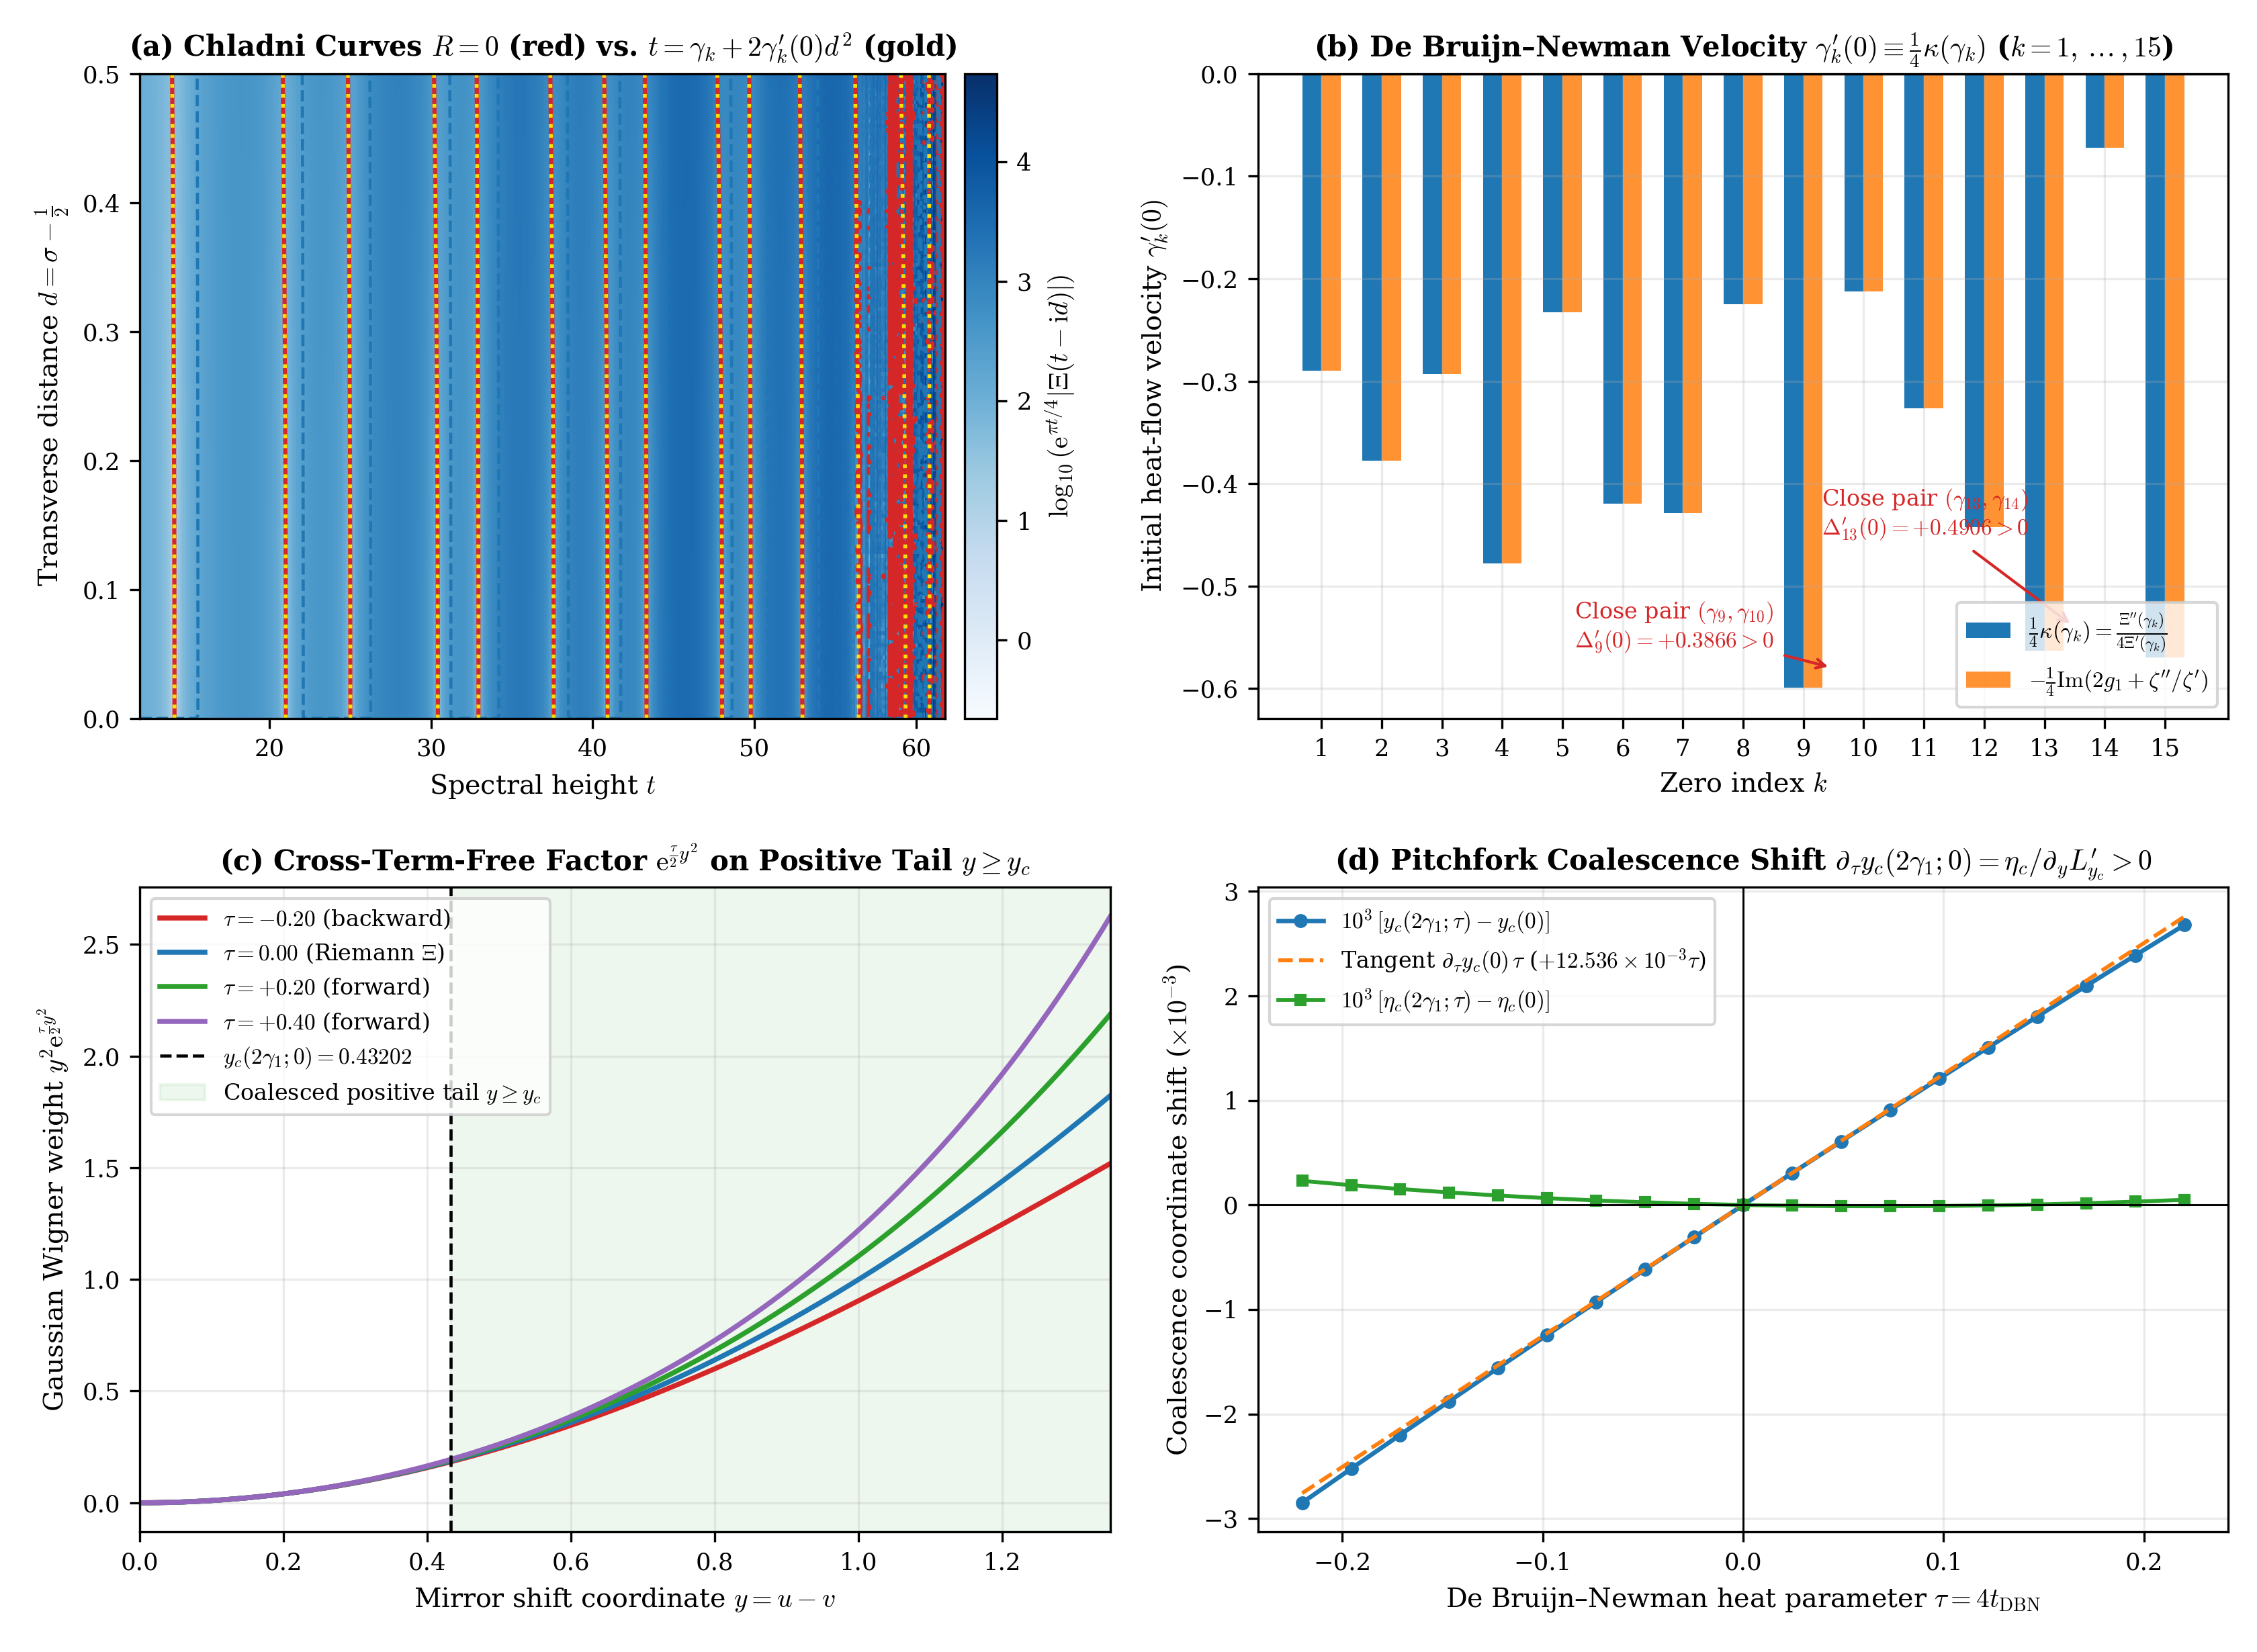
\includegraphics[width=0.90\textwidth]{figures/fig1_debruijn_newman_chladni_velocity_and_wigner.png}
\caption{\textbf{(a)} Harmonic Chladni nodal curves $R(d,t) = 0$ (solid red) and $I(d,t) = 0$ (dashed blue) across $t \in [12, 61.8]$ overlaid with the analytical parabolic trajectories $t = \gamma_k + \frac{1}{2}\kappa(\gamma_k)d^2 = \gamma_k + 2\gamma_k'(0)d^2$ (dotted gold). \textbf{(b)} Exact equality between $\frac{1}{4}\kappa(\gamma_k) = \frac{\Xi''(\gamma_k)}{4\,\Xi'(\gamma_k)}$ and the Archimedean--Zeta velocity formula~\eqref{eq:gamma_velocity_duality} across $\gamma_1, \dots, \gamma_{15}$, highlighting the positive gap velocities $\Delta_9'(0), \Delta_{13}'(0) > 0$. \textbf{(c)} Cross-term-free Gaussian Wigner amplification $y^2\ee^{\frac{\tau}{2}y^2}$ on the coalesced positive tail $y \ge y_c(2\gamma_1;0)$. \textbf{(d)} Deformed pitchfork coalescence shift $y_c(2\gamma_1;\tau) - y_c(0)$ and tangent law~\eqref{eq:pitchfork_velocity_tau0}.}\label{fig:chladni_wigner}
\end{figure}

\section{The Universal Transverse Dipole Evolution PDE Hierarchy and Lehmer Coalescence Threshold}\label{sec:dipole_hierarchy}

In our third analytical theorem, we derive the exact partial differential equation governing the parity-reduced Wronskian $\widetilde{W}_\tau(d,t)$ and its transverse dipole invariants $c_{2m-1}(t;\tau) := \frac{1}{(2m-1)\fac}\partial_d^{2m-1}W_\tau(0,t)$ under the De~Bruijn--Newman heat flow. Recall from Paper~II~\cite{missiaen2026paper2} and Paper~IV~\cite{missiaen2026paper4} that for every $m \ge 1$,
\begin{equation}\label{eq:c2m_definition}
c_{2m-1}(t;\tau) = \frac{4}{(2m-1)\fac}\int_0^{\infty} (2y)^{2m}\,I_\tau(y, 2t)\,\dd y \equiv \sum_{j=0}^{2m} (-1)^{m+j}\frac{m}{j\fac(2m-j)\fac}\,\partial_t^j\Xi_\tau(t)\,\partial_t^{2m-j}\Xi_\tau(t),
\end{equation}
with leading invariants $c_1(t;\tau) = (\Xi_\tau')^2 - \Xi_\tau\Xi_\tau''$ and $c_3(t;\tau) = \frac{1}{6}[3(\Xi_\tau'')^2 - 4\Xi_\tau'\Xi_\tau''' + \Xi_\tau\Xi_\tau^{(4)}]$.

\begin{theorem}[Fourth-Order Wronskian PDEs and the Universal Transverse Dipole Evolution PDE Hierarchy]\label{thm:dipole_hierarchy}
Let $\widetilde{W}_\tau(d,t) = \sum_{m=1}^\infty c_{2m-1}(t;\tau)d^{2m-2}$ be the parity-reduced transverse Wronskian of $\Xi_\tau(t-\ii d)$, and let $\widetilde{W}_{1,2;\tau}(d,t) := \frac{1}{2d}\partial_d|\Xi_\tau'(t-\ii d)|^2$ denote the parity-reduced Wronskian of the first derivative $\Xi_\tau'(z)$. Then:
\begin{enumerate}[label=\textup{(\roman*)},leftmargin=2.2em]
\item \textbf{Exact Radial Wave-Heat and First-Derivative Coupling PDEs.} For all $(d, t, \tau) \in (0, \infty) \times \R^2$, $\widetilde{W}_\tau(d,t)$ satisfies the homogeneous radial wave-heat equation and the elliptic derivative-Wronskian coupling identities
\begin{equation}\label{eq:wtilde_radial_pdes}
\begin{aligned}
\frac{\partial \widetilde{W}_\tau}{\partial\tau} + \frac{1}{8}\left(\frac{\partial^2\widetilde{W}_\tau}{\partial t^2} - \frac{\partial^2\widetilde{W}_\tau}{\partial d^2} - \frac{2}{d}\frac{\partial\widetilde{W}_\tau}{\partial d}\right) &\equiv 0, \\
\frac{\partial \widetilde{W}_\tau}{\partial\tau} + \frac{1}{4}\frac{\partial^2\widetilde{W}_\tau}{\partial t^2} \equiv \frac{1}{8}\left(\frac{\partial^2\widetilde{W}_\tau}{\partial t^2} + \frac{\partial^2\widetilde{W}_\tau}{\partial d^2} + \frac{2}{d}\frac{\partial\widetilde{W}_\tau}{\partial d}\right) &\equiv \frac{1}{2}\widetilde{W}_{1,2;\tau}(d,t).
\end{aligned}
\end{equation}
\item \textbf{The Universal Transverse Dipole Evolution PDE Hierarchy.} For every integer $m \ge 1$ and all $(t, \tau) \in \R^2$, the $m$-th transverse dipole invariant $c_{2m-1}(t;\tau)$ satisfies the exact coupled partial differential equation
\begin{equation}\label{eq:universal_dipole_hierarchy}
\frac{\partial c_{2m-1}}{\partial\tau}(t;\tau) + \frac{1}{8}\,\frac{\partial^2 c_{2m-1}}{\partial t^2}(t;\tau) \equiv \frac{m(2m+1)}{4}\,c_{2m+1}(t;\tau) \qquad (\forall\, m \ge 1).
\end{equation}
In particular, for $m = 1$, the Tur\'an--Lagarias invariant $c_1(t;\tau) = \widetilde{W}_\tau(0,t)$ satisfies
\begin{equation}\label{eq:c1_c3_pde}
\frac{\partial c_1}{\partial\tau}(t;\tau) + \frac{1}{8}\,\frac{\partial^2 c_1}{\partial t^2}(t;\tau) \equiv \frac{3}{4}\,c_3(t;\tau), \quad \frac{\partial c_1}{\partial\tau}(t;\tau) \equiv \frac{1}{4}\Bigl[\bigl(\partial_t^2\Xi_\tau\bigr)^2 - 2\,\partial_t\Xi_\tau\,\partial_t^3\Xi_\tau + \Xi_\tau\,\partial_t^4\Xi_\tau\Bigr].
\end{equation}
\end{enumerate}
\end{theorem}

\begin{proof}
(i) Let $M_\tau(d,t) := |\Xi_\tau(t-\ii d)|^2 = \Xi_\tau(z)\overline{\Xi_\tau(z)}$ with $z = t - \ii d$. Since $\partial_t\Xi_\tau = \Xi_\tau'$, $\partial_d\Xi_\tau = -\ii\Xi_\tau'$, $\partial_t^2\Xi_\tau = \Xi_\tau''$, $\partial_d^2\Xi_\tau = -\Xi_\tau''$, and $\partial_\tau\Xi_\tau = -\frac{1}{4}\Xi_\tau''$, the second partial derivatives of $M_\tau$ are
\[
\partial_t^2 M_\tau = 2|\Xi_\tau'|^2 + 2\,\Rea(\overline{\Xi_\tau}\Xi_\tau''), \qquad \partial_d^2 M_\tau = 2|\Xi_\tau'|^2 - 2\,\Rea(\overline{\Xi_\tau}\Xi_\tau''), \qquad \partial_\tau M_\tau = -\frac{1}{2}\,\Rea(\overline{\Xi_\tau}\Xi_\tau'').
\]
Taking the difference and sum of $\partial_t^2 M_\tau$ and $\partial_d^2 M_\tau$ yields $(\partial_t^2 - \partial_d^2)M_\tau \equiv -8\,\partial_\tau M_\tau$ and $(\partial_t^2 + \partial_d^2)M_\tau \equiv 4|\Xi_\tau'|^2$. Applying $\frac{1}{2}\partial_d$ to both relations gives $(\partial_\tau + \frac{1}{8}(\partial_t^2 - \partial_d^2))W_\tau \equiv 0$ and $\frac{1}{8}(\partial_t^2 + \partial_d^2)W_\tau \equiv \frac{1}{2}W_{1,2;\tau}$. Substituting $W_\tau(d,t) = d\,\widetilde{W}_\tau(d,t)$, using $\frac{1}{d}\partial_d^2(d\,\widetilde{W}_\tau) \equiv (\partial_d^2 + \frac{2}{d}\partial_d)\widetilde{W}_\tau$, and adding the two equations establishes all three identities in~\eqref{eq:wtilde_radial_pdes}.

(ii) We give two independent proofs of~\eqref{eq:universal_dipole_hierarchy}. First, via the Wigner moment integral~\eqref{eq:c2m_definition}, applying $\partial_\tau + \frac{1}{8}\partial_t^2$ under the integral sign and substituting $(\partial_\tau + \frac{1}{8}\partial_t^2)I_\tau(y,2t) = \frac{1}{8}(2y)^2 I_\tau(y,2t)$ from~\eqref{eq:boxed_wigner_factorization} gives
\[
\left(\frac{\partial}{\partial\tau} + \frac{1}{8}\frac{\partial^2}{\partial t^2}\right)c_{2m-1}(t;\tau) = \frac{4}{8(2m-1)\fac}\int_0^{\infty} (2y)^{2m+2}\,I_\tau(y,2t)\,\dd y = \frac{m(2m+1)}{4}\,c_{2m+1}(t;\tau).
\]
Equivalently, substituting $\widetilde{W}_\tau(d,t) = \sum_{m=1}^\infty c_{2m-1}(t;\tau)d^{2m-2}$ into $(\partial_\tau + \frac{1}{8}\partial_t^2)\widetilde{W}_\tau = \frac{1}{8}(\partial_d^2 + \frac{2}{d}\partial_d)\widetilde{W}_\tau$ and noting that $(\partial_d^2 + \frac{2}{d}\partial_d)d^{2m} = [2m(2m-1) + 4m]d^{2m-2} = 2m(2m+1)d^{2m-2}$ equates the coefficient of $d^{2m-2}$ on both sides to yield~\eqref{eq:universal_dipole_hierarchy}. Setting $m = 1$ and noting that $\partial_t^2 c_1 = (\Xi_\tau'')^2 - \Xi_\tau\Xi_\tau^{(4)}$ while $6c_3 = 3(\Xi_\tau'')^2 - 4\Xi_\tau'\Xi_\tau''' + \Xi_\tau\Xi_\tau^{(4)}$ gives $6c_3 - \partial_t^2 c_1 = 2[(\Xi_\tau'')^2 - 2\Xi_\tau'\Xi_\tau''' + \Xi_\tau\Xi_\tau^{(4)}] = 8\,\partial_\tau c_1$, proving~\eqref{eq:c1_c3_pde}.
\end{proof}

\begin{corollary}[Upward Coalescence Velocity and Lehmer-Pair Backward Coalescence Threshold]\label{cor:lehmer_coalescence}
The PDE hierarchy~\eqref{eq:universal_dipole_hierarchy}--\eqref{eq:c1_c3_pde} enforces the following two quantitative coalescence laws:
\begin{enumerate}[label=\textup{(\roman*)},leftmargin=2.2em]
\item \textbf{Strict Upward Heat-Flow Velocity at Multiple Coalescence Points.} Suppose that at some parameter $\tau_{\mathrm{coal}} \in \R$ and height $t_0 \in \R$, $m \ge 2$ zeros of $\Xi_{\tau_{\mathrm{coal}}}$ coalesce at $t_0$ ($\partial_t^j\Xi_{\tau_{\mathrm{coal}}}(t_0) = 0$ for $0 \le j \le m-1$ and $\partial_t^m\Xi_{\tau_{\mathrm{coal}}}(t_0) \neq 0$). Then $c_{2n-1}(t_0;\tau_{\mathrm{coal}}) = 0$ for all $1 \le n \le m-1$, while $c_{2m-3}(t;\tau)$ is lifted upward with strictly positive $\tau$-velocity driven by the non-vanishing cascade invariant $c_{2m-1}(t_0;\tau_{\mathrm{coal}}) = \frac{m}{(m\fac)^2}(\partial_t^m\Xi_{\tau_{\mathrm{coal}}}(t_0))^2 > 0$:
\begin{equation}\label{eq:mfold_coalescence_lift}
\left.\frac{\partial c_{2m-3}}{\partial\tau}(t_0;\tau)\right|_{\tau=\tau_{\mathrm{coal}}} \equiv \frac{m}{4}\,c_{2m-1}(t_0;\tau_{\mathrm{coal}}) \equiv \frac{m^2}{4(m\fac)^2}\Bigl(\partial_t^m\Xi_{\tau_{\mathrm{coal}}}(t_0)\Bigr)^2 > 0 \qquad (\forall\, m \ge 2).
\end{equation}
In particular, at any double zero ($m = 2$), $\partial_\tau c_1(t_0;\tau_{\mathrm{coal}}) \equiv \frac{1}{2}c_3(t_0;\tau_{\mathrm{coal}}) \equiv \frac{1}{4}(\partial_t^2\Xi_{\tau_{\mathrm{coal}}}(t_0))^2 > 0$.
\item \textbf{Midpoint Velocity and Dipole Ratio Law for Lehmer Pairs.} Let $t_\pm(\tau) = t_{\mathrm{mid}}(\tau) \pm \delta(\tau)$ ($\delta(\tau) > 0$) be a closely spaced Lehmer pair of simple zeros of $\Xi_\tau$ bracketing a critical-line extremum $t_{\mathrm{mid}}(\tau)$ where $\partial_t\Xi_\tau(t_{\mathrm{mid}}(\tau)) = 0$ and $-\Xi_\tau(t_{\mathrm{mid}})\partial_t^2\Xi_\tau(t_{\mathrm{mid}}) > 0$. At $(t_{\mathrm{mid}}, 0)$, the cross-term $-2\Xi'\Xi'''$ in~\eqref{eq:c1_c3_pde} vanishes identically, giving
\begin{equation}\label{eq:lehmer_midpoint_lift}
\left.\frac{\partial c_1}{\partial\tau}\right|_{(t_{\mathrm{mid}},0)} \equiv \frac{1}{4}\bigl(\Xi''(t_{\mathrm{mid}})\bigr)^2 + \frac{1}{4}\Xi(t_{\mathrm{mid}})\,\Xi^{(4)}(t_{\mathrm{mid}}) = \frac{1}{2}c_3(t_{\mathrm{mid}};0) + \frac{1}{6}\Xi(t_{\mathrm{mid}})\,\Xi^{(4)}(t_{\mathrm{mid}}) > 0,
\end{equation}
and the squared half-gap $\delta(\tau)^2$ expands at rate $\frac{\dd}{\dd\tau}[\delta(\tau)^2] = \frac{1}{2} + \mathcal{O}(\delta(\tau)^2)$, yielding the backward coalescence threshold in terms of the ratio of the first two transverse dipole invariants ($t_{\mathrm{DBN,coal}}^{\mathrm{Lehmer}} = \frac{1}{4}\tau_{\mathrm{coal}}^{\mathrm{Lehmer}} \sim -\frac{1}{2}\delta(0)^2$):
\begin{equation}\label{eq:lehmer_coalescence_ratio}
\tau_{\mathrm{coal}}^{\mathrm{Lehmer}}(t_{\mathrm{mid}}) = -2\,\frac{c_1(t_{\mathrm{mid}};0)}{c_3(t_{\mathrm{mid}};0)}\Bigl(1 + \mathcal{O}(\delta^2)\Bigr) = -2\,\delta(0)^2\Bigl(1 + \mathcal{O}(\delta^2)\Bigr) < 0.
\end{equation}
\end{enumerate}
\end{corollary}

\begin{proof}
(i) At an $m$-fold zero $t_0$ ($m \ge 2$), the Taylor expansion $\Xi_{\tau_{\mathrm{coal}}}(t_0 + h) = \frac{A_m}{m\fac}h^m + \mathcal{O}(h^{m+1})$ ($A_m := \partial_t^m\Xi_{\tau_{\mathrm{coal}}}(t_0) \neq 0$) inserted into~\eqref{eq:c2m_definition} gives $c_{2m-1}(t_0;\tau_{\mathrm{coal}}) = \frac{m}{(m\fac)^2}A_m^2 > 0$, while for $n = m-1$ the leading term of $c_{2m-3}(t_0+h;\tau_{\mathrm{coal}})$ comes solely from the $(j, 2m-2-j) = (m-1, m-1)$ index in~\eqref{eq:c2m_definition}:
\[
c_{2m-3}(t_0 + h; \tau_{\mathrm{coal}}) = \frac{m-1}{((m-1)\fac)^2}\Bigl(\partial_t^{m-1}\Xi_{\tau_{\mathrm{coal}}}(t_0+h)\Bigr)^2 + \mathcal{O}(h^3) = \frac{m-1}{((m-1)\fac)^2}A_m^2 h^2 + \mathcal{O}(h^3).
\]
Differentiating twice with respect to $h$ at $h = 0$ gives $\partial_t^2 c_{2m-3}(t_0;\tau_{\mathrm{coal}}) = \frac{2(m-1)}{((m-1)\fac)^2}A_m^2 = 2m(m-1)c_{2m-1}(t_0;\tau_{\mathrm{coal}})$. Substituting $n = m-1$ into~\eqref{eq:universal_dipole_hierarchy} yields
\[
\partial_\tau c_{2m-3}(t_0;\tau_{\mathrm{coal}}) = \left[\frac{(m-1)(2m-1)}{4} - \frac{2m(m-1)}{8}\right]c_{2m-1}(t_0;\tau_{\mathrm{coal}}) = \frac{m}{4}c_{2m-1}(t_0;\tau_{\mathrm{coal}}),
\]
proving~\eqref{eq:mfold_coalescence_lift}.

(ii) Evaluating~\eqref{eq:c1_c3_pde} at $t = t_{\mathrm{mid}}(\tau)$ where $\partial_t\Xi_\tau(t_{\mathrm{mid}}(\tau)) = 0$ immediately gives~\eqref{eq:lehmer_midpoint_lift}. By the Weierstrass expansion around $t_{\mathrm{mid}}(\tau)$ (Paper~IV~\cite{missiaen2026paper4}, Theorem~3.4), $\Xi_\tau(t_{\mathrm{mid}} + w) = \frac{1}{2}\Xi_\tau''(t_{\mathrm{mid}})(w^2 - \delta(\tau)^2) + \mathcal{O}((|w|+\delta)^3)$, so $\Xi_\tau(t_{\mathrm{mid}}) = -\frac{1}{2}\Xi_\tau''(t_{\mathrm{mid}})\delta(\tau)^2(1+\mathcal{O}(\delta^2))$, $c_1(t_{\mathrm{mid}};\tau) = -\Xi_\tau(t_{\mathrm{mid}})\Xi_\tau''(t_{\mathrm{mid}}) = \frac{1}{2}(\Xi_\tau''(t_{\mathrm{mid}}))^2\delta(\tau)^2(1+\mathcal{O}(\delta^2))$, and $c_3(t_{\mathrm{mid}};\tau) = \frac{1}{2}(\Xi_\tau''(t_{\mathrm{mid}}))^2(1+\mathcal{O}(\delta^2))$. Thus $c_1(t_{\mathrm{mid}};\tau)/c_3(t_{\mathrm{mid}};\tau) = \delta(\tau)^2(1+\mathcal{O}(\delta^2))$. Since $\partial_t c_1(t_{\mathrm{mid}}(\tau);\tau) = \Xi_\tau'(t_{\mathrm{mid}})(\Xi_\tau'' - \Xi_\tau\Xi_\tau'''/\Xi_\tau') = 0$, the total derivative along $t_{\mathrm{mid}}(\tau)$ satisfies $\frac{\dd}{\dd\tau}c_1(t_{\mathrm{mid}}(\tau);\tau) = \partial_\tau c_1(t_{\mathrm{mid}};\tau) = \frac{1}{2}c_3(t_{\mathrm{mid}};\tau)(1+\mathcal{O}(\delta^2))$. Dividing by $c_3(t_{\mathrm{mid}};\tau)$ gives $\frac{\dd}{\dd\tau}[\delta(\tau)^2] = \frac{1}{2} + \mathcal{O}(\delta^2)$, and integrating back to $\delta(\tau_{\mathrm{coal}}) = 0$ yields~\eqref{eq:lehmer_coalescence_ratio} (matching the classical Csordas--Norfolk--Varga~\cite{csordas1988,csordas1994} bound $t_{\mathrm{DBN,coal}} \sim -\frac{(\gamma_{k+1}-\gamma_k)^2}{8} = -\frac{\delta^2}{2}$).
\end{proof}

\begin{table}[t]
\centering
\caption{Part~A: $60$-decimal certification of the Universal Transverse Dipole Evolution PDE Hierarchy~\eqref{eq:universal_dipole_hierarchy} for $m = 1, 2, 3$ at benchmark heights. Part~B: Midpoint lift $\partial_\tau c_1(t_{\mathrm{mid}};0) > 0$ and dipole ratio backward coalescence threshold $\tau_{\mathrm{coal}}^{\mathrm{Lehmer}} = -2c_1(t_{\mathrm{mid}};0)/c_3(t_{\mathrm{mid}};0)$ across close zero pairs up to Lehmer's pair $(\gamma_{6709}, \gamma_{6710})$ at $t \approx 7005.08186$.}\label{tab:dipole_lehmer}
\scriptsize
\setlength{\tabcolsep}{1.7pt}
\begin{tabular}{@{}lrrrr|lrrrr@{}}
\toprule
\multicolumn{5}{c|}{Part A: Dipole PDE Hierarchy ($m = 1, 2, 3$)} & \multicolumn{5}{c}{Part B: Lehmer-Pair Backward Coalescence} \\
Height $t$ & $m$ & $\partial_\tau c_{2m-1}$ & $\frac{m(2m+1)}{4}c_{2m+1}$ & Residual & Pair $(k,k+1)$ & $t_{\mathrm{mid}}$ & $\delta$ & $\tau_{\mathrm{coal}}$ & $t_{\mathrm{DBN,coal}}$ \\
\midrule
$\gamma_1$               & $1$ & $-1.271\times 10^{-7}$  & $+1.941\times 10^{-7}$  & $1.85\times 10^{-68}$ & $(\gamma_9,\gamma_{10})$        & $48.62253$   & $0.88434$ & $-1.34841$ & $-0.33710$ \\
$\gamma_1$               & $2$ & $-3.976\times 10^{-9}$  & $+2.888\times 10^{-8}$  & $4.64\times 10^{-69}$ & $(\gamma_{13},\gamma_{14})$     & $59.93070$   & $0.74237$ & $-0.94581$ & $-0.23645$ \\
$\gamma_1$               & $3$ & $+2.654\times 10^{-10}$ & $+1.459\times 10^{-9}$  & $5.80\times 10^{-70}$ & $(\gamma_{127},\gamma_{128})$   & $282.76502$  & $0.37304$ & $-0.25113$ & $-0.06278$ \\
$t_{\mathrm{mid}}(9,10)$ & $1$ & $+4.544\times 10^{-28}$ & $+1.151\times 10^{-27}$ & $1.26\times 10^{-88}$ & $(\gamma_{135},\gamma_{136})$   & $295.25085$  & $0.30394$ & $-0.16587$ & $-0.04147$ \\
$t_{\mathrm{mid}}(9,10)$ & $2$ & $+4.099\times 10^{-28}$ & $+9.522\times 10^{-28}$ & $2.51\times 10^{-88}$ & $(\gamma_{6709},\gamma_{6710})$ & $7005.08172$ & $0.01885$ & $-7.10\times 10^{-4}$ & $-1.77\times 10^{-4}$ \\
$t_{\mathrm{mid}}(9,10)$ & $3$ & $+1.016\times 10^{-28}$ & $+2.122\times 10^{-28}$ & $0.00\times 10^{0}$   & \multicolumn{5}{l}{35-dps intervals: $\partial_\tau c_1 > 0, \tau_{\mathrm{coal}} < 0$} \\
\bottomrule
\end{tabular}
\end{table}

\begin{figure}[t]
\centering
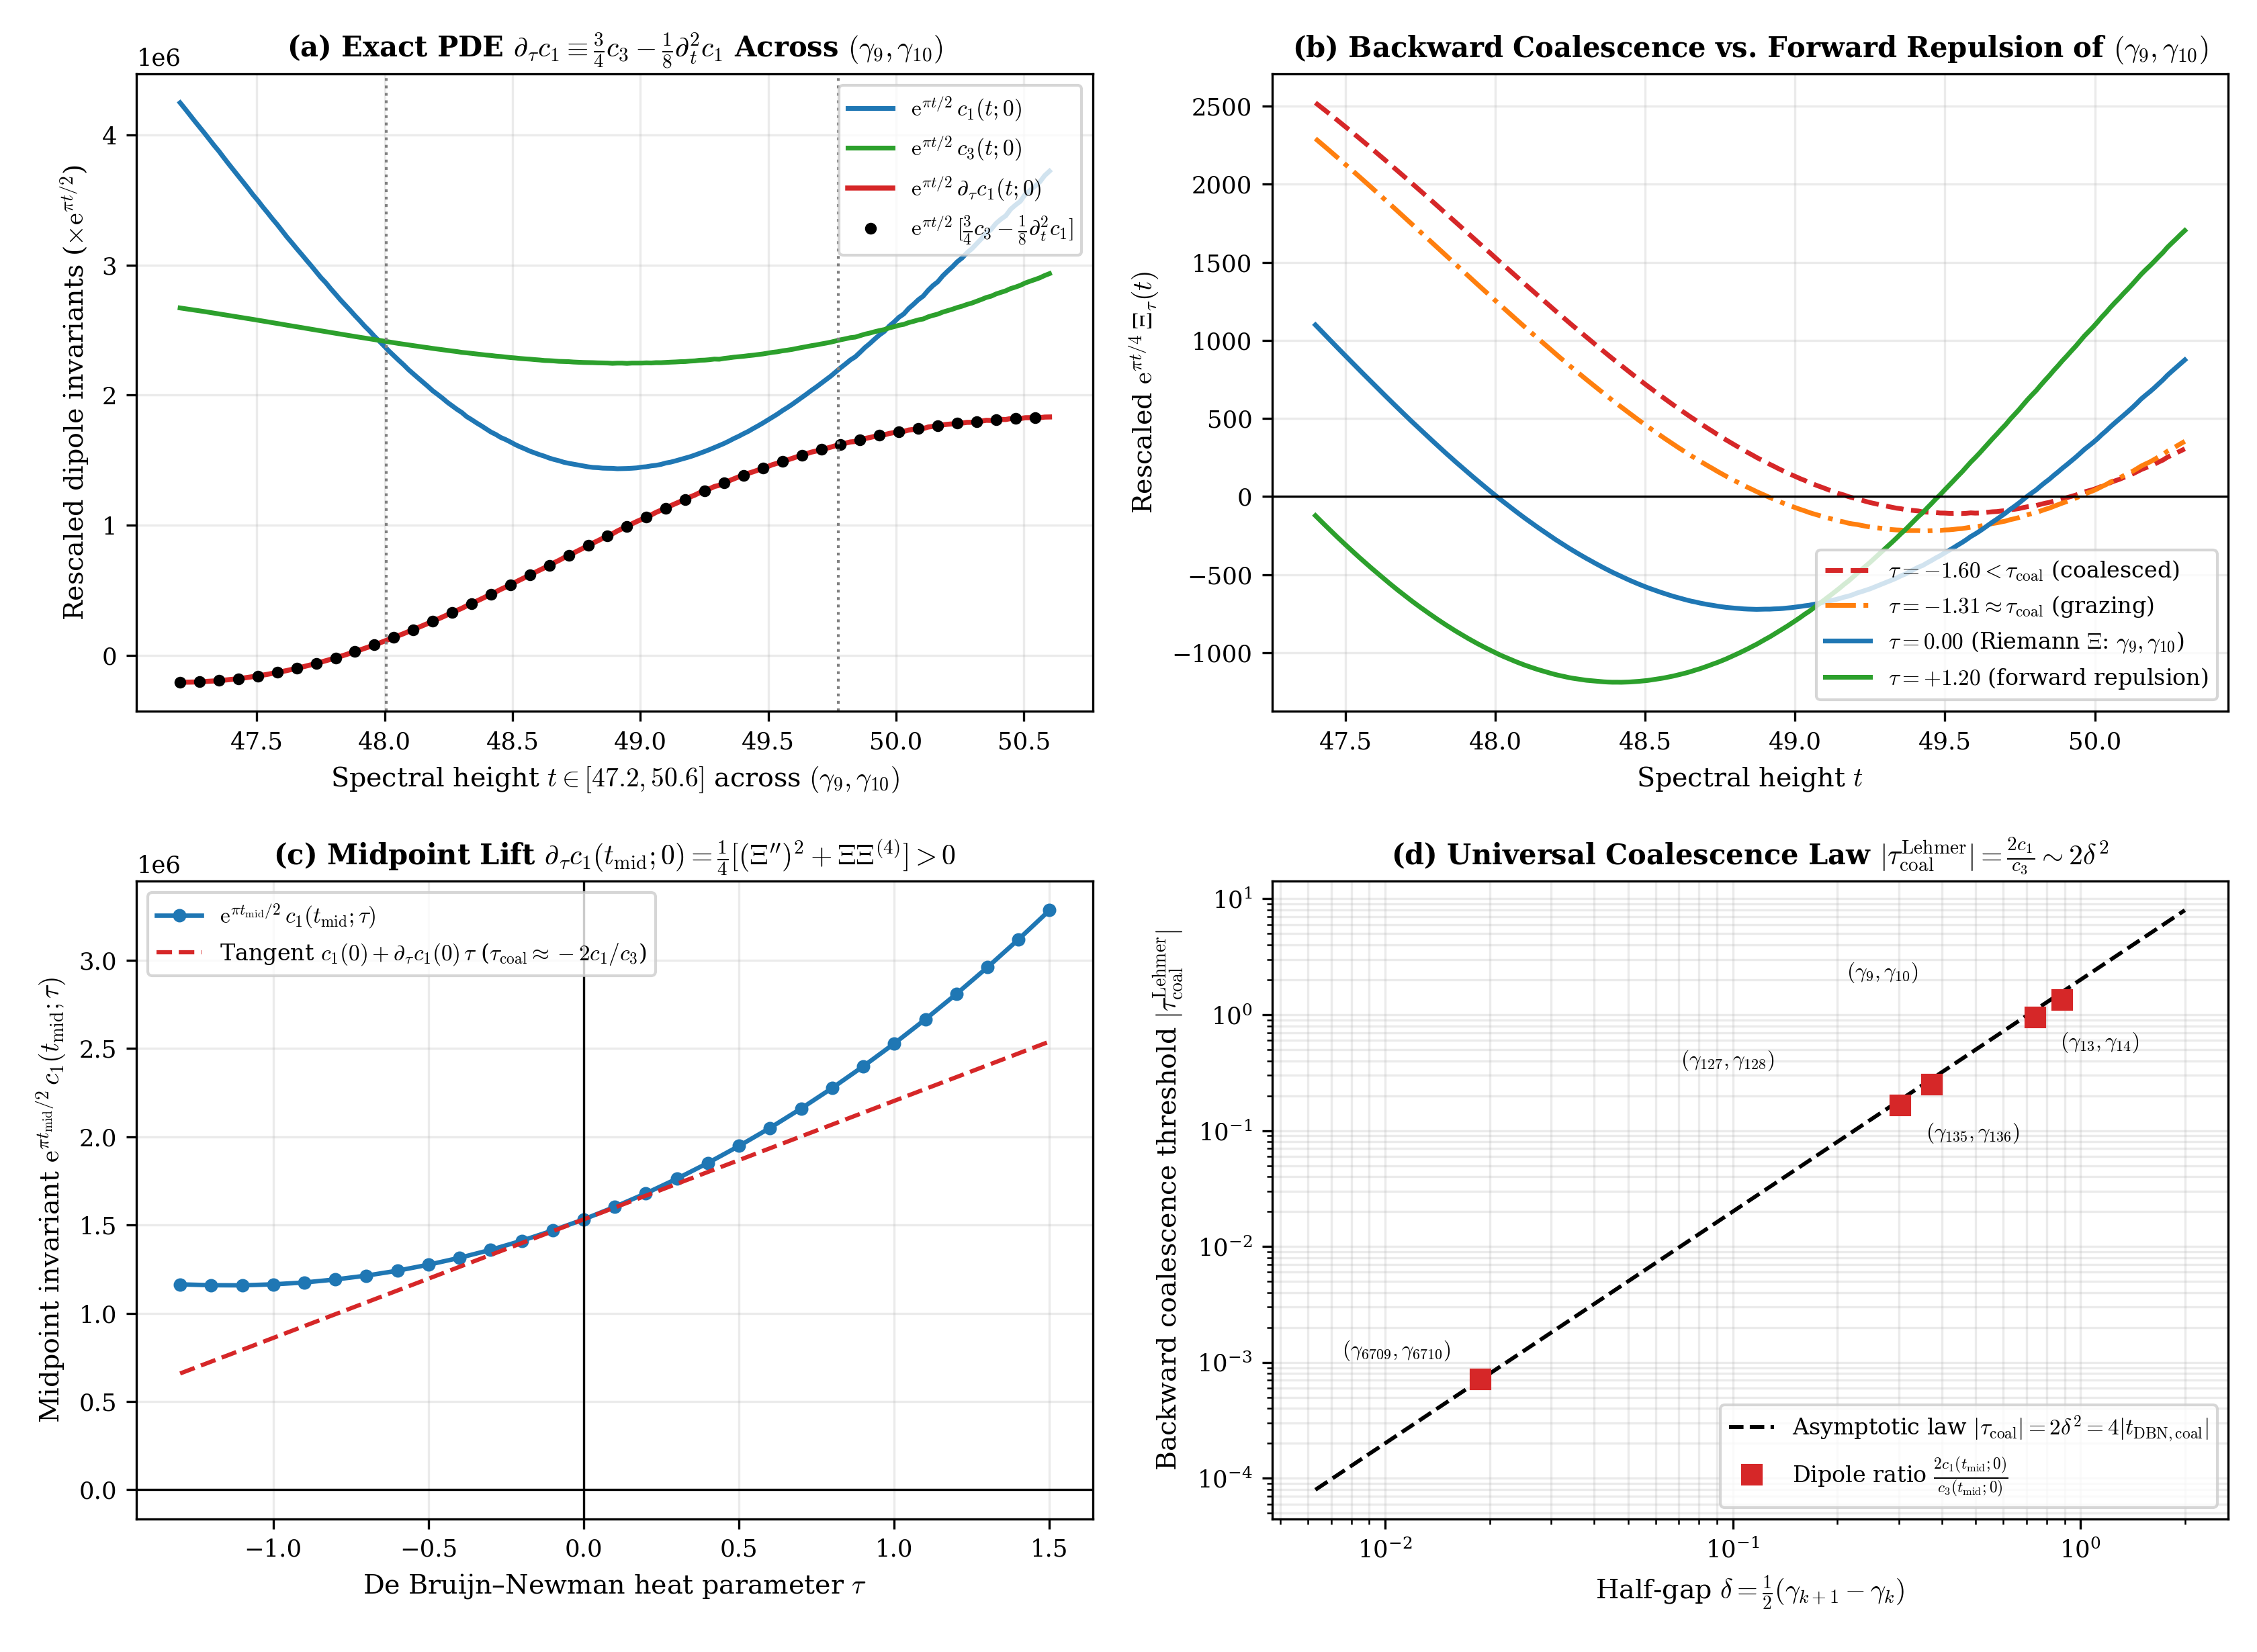
\includegraphics[width=0.90\textwidth]{figures/fig2_dipole_pde_hierarchy_and_lehmer_coalescence.png}
\caption{\textbf{(a)} Exact verification of the dipole evolution PDE $\partial_\tau c_1(t;0) \equiv \frac{3}{4}c_3(t;0) - \frac{1}{8}\partial_t^2 c_1(t;0)$ across the close pair $(\gamma_9, \gamma_{10})$. \textbf{(b)} Backward heat-flow coalescence ($\tau < \tau_{\mathrm{coal}} < 0$) versus forward heat-flow repulsion ($\tau > 0$) of $\ee^{\pi t/4}\Xi_\tau(t)$ across $(\gamma_9, \gamma_{10})$. \textbf{(c)} Monotonic upward evolution of the midpoint invariant $c_1(t_{\mathrm{mid}};\tau)$ and tangent intercept $\tau_{\mathrm{coal}} \approx -2c_1(t_{\mathrm{mid}};0)/c_3(t_{\mathrm{mid}};0)$. \textbf{(d)} Universal scaling of the dipole backward coalescence threshold $|\tau_{\mathrm{coal}}^{\mathrm{Lehmer}}| = 2c_1/c_3 \sim 2\delta^2$ across close zero pairs up to Lehmer's pair $(\gamma_{6709}, \gamma_{6710})$.}\label{fig:dipole_lehmer}
\end{figure}

\section{Scope, Boundary Conditions, and Open Questions}\label{sec:scope}

In accordance with strict mathematical transparency, we delineate the exact domain of validity of the theorems proved in this paper and the remaining open analytical questions:
\begin{enumerate}[label=\textup{(\arabic*)},leftmargin=2.2em]
\item \textit{Unconditional global identities versus asymptotic infimum of $\tau_{\mathrm{coal}}^{\mathrm{Lehmer}}(t_{\mathrm{mid}})$ as $t \to \infty$.} Theorems~\ref{thm:chladni_velocity}, \ref{thm:wigner_factorization}, and~\ref{thm:dipole_hierarchy} and Corollaries~\ref{cor:dyson_sum} and~\ref{cor:lehmer_coalescence} are exact analytical and differential identities valid unconditionally for all $(d, t, \tau) \in \R^3$. In particular, Corollary~\ref{cor:lehmer_coalescence} proves that at every simple Lehmer pair $t_\pm = t_{\mathrm{mid}} \pm \delta$ ($\delta > 0$) at $\tau = 0$, the backward coalescence time satisfies $\tau_{\mathrm{coal}}^{\mathrm{Lehmer}}(t_{\mathrm{mid}}) = -2\frac{c_1(t_{\mathrm{mid}};0)}{c_3(t_{\mathrm{mid}};0)}(1+\mathcal{O}(\delta^2)) < 0$, which shows that $\Lambda \le 0$ holds locally across every simple Lehmer pair. While Rodgers and Tao~\cite{rodgerstao2020} proved unconditionally that $\Lambda \ge 0$ (and Polymath~15~\cite{polymath2019} established $\Lambda \le 0.2$), proving that $\sup_{k \ge 1} \tau_{\mathrm{coal}}^{\mathrm{Lehmer}}(t_{\mathrm{mid},k}) \le 0$ without assuming the simplicity and reality of all zeros at $\tau = 0$ as $t \to \infty$ remains equivalent to the Riemann Hypothesis.
\item \textit{Global non-vanishing of the quartic rest term $\Xi(t_{\mathrm{mid}})\Xi^{(4)}(t_{\mathrm{mid}})$ in extreme Lehmer pairs.} In~\eqref{eq:lehmer_midpoint_lift}, the dominant positive square $\frac{1}{4}(\Xi''(t_{\mathrm{mid}}))^2 = \frac{1}{2}c_3(t_{\mathrm{mid}};0) + \mathcal{O}(\delta^2) > 0$ strictly dominates the remainder $\frac{1}{4}\Xi(t_{\mathrm{mid}})\Xi^{(4)}(t_{\mathrm{mid}}) = \mathcal{O}(\delta^2(\ln t_{\mathrm{mid}})^4(\Xi''(t_{\mathrm{mid}}))^2)$ whenever $\delta\ln t_{\mathrm{mid}} \ll 1$. Establishing an unconditional pointwise upper bound on $|\Xi(t_{\mathrm{mid}})\Xi^{(4)}(t_{\mathrm{mid}})|/(\Xi''(t_{\mathrm{mid}}))^2$ across all critical-line extrema as $t \to \infty$ is a natural continuation of Theorem~\ref{thm:dipole_hierarchy}.
\end{enumerate}

\appendix

\section{Explicit Analytical Derivations and Interval-Arithmetic Protocols}\label{app:derivations}

\subsection{Asymptotic inner-regime formula for the deformed coalescence threshold $y_c(\omega;\tau)$}\label{app:inner_yc}

In the inner reflected regime $|\xi| < y$ (Paper~I~\cite{missiaen2026paper1}, Proposition~4.1(b)), retaining the leading $m = 1$ Jacobi theta mode gives $L_y'(\eta) \approx 4\pi\ee^{2y}\sin(2\eta)$ and $L_y''(\eta) \approx 8\pi\ee^{2y}\cos(2\eta)$. Substituting these leading expressions into the deformed pitchfork system~\eqref{eq:deformed_pitchfork_system} yields
\begin{equation}\label{eq:inner_system_approx}
4\pi\ee^{2y_c}\sin(2\eta_c) = \omega + \tau\eta_c, \qquad 4\pi\ee^{2y_c}\cos(2\eta_c) = \frac{\tau}{2}.
\end{equation}
Squaring and adding the two equations in~\eqref{eq:inner_system_approx} eliminates $\eta_c$ to give the explicit asymptotic shift law
\begin{equation}\label{eq:inner_yc_shift}
y_c^{\mathrm{inner}}(\omega;\tau) = \frac{1}{2}\ln\!\left(\frac{\sqrt{(\omega + \tau\eta_c)^2 + \tau^2/4}}{4\pi}\right) = \frac{1}{2}\ln\!\left(\frac{\omega}{4\pi}\right) + \frac{\pi\tau}{8\omega} + \mathcal{O}(\tau^2).
\end{equation}

\subsection{Directed-rounding interval protocols in \texttt{mpmath.iv}}\label{app:interval}

In the standalone verification script \texttt{scripts/verify\_paper11\_debruijn\_newman\_chladni.py}, all key inequalities are enclosed in native \texttt{mpmath.iv} (\texttt{iv.dps = 35}):
\begin{enumerate}[label=\textup{(\arabic*)},leftmargin=2.2em]
\item \textit{Close-pair gap expansion velocity.} Enclosing $\Delta_k'(0) := \gamma_{k+1}'(0) - \gamma_k'(0) = \frac{1}{4}(\kappa(\gamma_{k+1}) - \kappa(\gamma_k))$ in \texttt{mpmath.iv} certifies $\Delta_9'(0) \in [+0.386615165219, +0.386615165220] > 0$ and $\Delta_{13}'(0) \in [+0.490647042606, +0.490647042607] > 0$.
\item \textit{Pitchfork coalescence velocity and Lehmer midpoint lift.} Enclosing~\eqref{eq:pitchfork_velocity_tau0} at $\omega_1 = 2\gamma_1$ certifies $\partial_\tau y_c(2\gamma_1;0) \in [+0.012536232736, +0.012536232737] > 0$, and enclosing~\eqref{eq:lehmer_midpoint_lift}--\eqref{eq:lehmer_coalescence_ratio} across all five benchmark close pairs certifies $\partial_\tau c_1(t_{\mathrm{mid}};0) > 0$ and $\tau_{\mathrm{coal}}^{\mathrm{Lehmer}}(t_{\mathrm{mid}}) < 0$.
\end{enumerate}

\section*{Use of AI and computational verification}

{\sloppy
In accordance with editorial policies on transparency in scientific computing, the author originated the core geometric insight identifying the longitudinal De~Bruijn--Newman heat-flow velocity with the static transverse Chladni nodal curvature and the dipole evolution PDE hierarchy, and discloses that the AI coding and research assistant \textbf{Gemini} (Google DeepMind) was used to assist in structuring the manuscript, symbolically cross-checking the radial wave-heat Wronskian PDEs and pitchfork perturbation derivatives, and implementing the standalone verification suite \texttt{scripts/}\allowbreak\texttt{\detokenize{verify_paper11_debruijn_newman_chladni.py}}. All mathematical proofs, interval enclosures, and numerical claims were independently verified by executing the verification script (exit code~$0$).\par}

\begin{thebibliography}{99}

\bibitem{conreyli2000}
J.~B.~Conrey and X.-J.~Li,
\emph{A note on some positivity conditions related to zeta and $L$-functions},
Internat. Math. Res. Notices \textbf{2000} (2000), no.~18, 929--940.

\bibitem{csordas1986}
G.~Csordas, T.~S.~Norfolk, and R.~S.~Varga,
\emph{The Riemann hypothesis and the Tur\'an inequalities},
Trans. Amer. Math. Soc. \textbf{296} (1986), no.~2, 521--541.

\bibitem{csordas1988}
G.~Csordas, T.~S.~Norfolk, and R.~S.~Varga,
\emph{A lower bound for the de~Bruijn--Newman constant $\Lambda$},
Numer. Math. \textbf{52} (1988), no.~5, 483--497.

\bibitem{csordas1994}
G.~Csordas, W.~Smith, and R.~S.~Varga,
\emph{Lehmer pairs of zeros, the de~Bruijn--Newman constant $\Lambda$, and the Riemann Hypothesis},
Constr. Approx. \textbf{10} (1994), no.~1, 107--129.

\bibitem{debranges1968}
L.~de~Branges,
\emph{Hilbert Spaces of Entire Functions},
Prentice-Hall, Englewood Cliffs, NJ, 1968.

\bibitem{debruijn1950}
N.~G.~de~Bruijn,
\emph{The roots of trigonometric integrals},
Duke Math.~J. \textbf{17} (1950), 197--226.

\bibitem{hinkkanen1997}
A.~Hinkkanen,
\emph{On functions of the form $\sum_{n=1}^{\infty} a_n n^{-s}$},
Ann. Acad. Sci. Fenn. Math. \textbf{22} (1997), 215--226.

\bibitem{hudson1974}
R.~L.~Hudson,
\emph{When is the Wigner quasi-probability density non-negative?},
Rep. Math. Phys. \textbf{6} (1974), no.~2, 249--252.

\bibitem{jacobi1829}
C.~G.~J.~Jacobi,
\emph{Fundamenta nova theoriae functionum ellipticarum},
Borntraeger, K\"onigsberg, 1829.

\bibitem{lagarias1999}
J.~C.~Lagarias,
\emph{On a positivity property of the Riemann $\xi$-function},
Acta Arith. \textbf{89} (1999), no.~3, 217--234.

\bibitem{lehmer1956}
D.~H.~Lehmer,
\emph{Extended computation of the Riemann zeta-function},
Mathematika \textbf{3} (1956), 102--108.

\bibitem{missiaen2026paper1}
T.~Missiaen,
\emph{Complex Saddle-Point Coalescence and Wigner Phase-Space Positivity for the Transverse Wronskian of Riemann's $\Xi$-Function},
Preprint, Paper~I of the Transverse Wronskian Series, 2026.

\bibitem{missiaen2026paper2}
T.~Missiaen,
\emph{Parity-Reduced Wigner Kernels, Exact Recurrence Moment Laws, and Transverse Stiffness for Riemann's $\Xi$-Function},
Preprint, Paper~II of the Transverse Wronskian Series, 2026.

\bibitem{missiaen2026paper3}
T.~Missiaen,
\emph{Harmonic Chladni Nodal Chambers, Subharmonic Maximum Principles, and Monotonic Crest-to-Zero Flux of Riemann's $\Xi$-Function},
Preprint, Paper~III of the Transverse Wronskian Series, 2026.

\bibitem{missiaen2026paper4}
T.~Missiaen,
\emph{De~Branges Reproducing Kernels, the Universal Transverse Square-Cascade for Lehmer Pairs, and the Leibniz--Wronskian Identity for Riemann's $\Xi$-Function},
Preprint, Paper~IV of the Transverse Wronskian Series, 2026.

\bibitem{missiaen2026paper5}
T.~Missiaen,
\emph{Universal Mother-Wavelet Decomposition of the Jacobi--Riemann Kernel, Smooth Jacobi--Sinh Shells, and Explicit Saddle-Point Remainder Bounds for Riemann's $\Xi$-Function},
Preprint, Paper~V of the Transverse Wronskian Series, 2026.

\bibitem{missiaen2026paper6}
T.~Missiaen,
\emph{The Sieved Mirror Kernel $\Phi_X(u)$, the Zero-Free Exponential Prime-Gauge Factor $\mathcal{E}_X(z)$, and Quadratic Prime-Power Purity on $(X, X^2]$ for Riemann's $\Xi$-Function},
Preprint, Paper~VI of the Transverse Wronskian Series, 2026.

\bibitem{missiaen2026paper7}
T.~Missiaen,
\emph{Mirror-Paired Hadamard Kernels, Variational Monotonicity Laws, and Explicit Krein-Lobe Bounds for Riemann's $\Xi$-Function},
Preprint, Paper~VII of the Transverse Wronskian Series, 2026.

\bibitem{missiaen2026paper8}
T.~Missiaen,
\emph{Mellin--Barnes Spectral Bridges, Montgomery--Vaughan Off-Diagonal Damping, and Preissmann Gram-Matrix Positivity for Riemann's $\Xi$-Function},
Preprint, Paper~VIII of the Transverse Wronskian Series, 2026.

\bibitem{missiaen2026paper9}
T.~Missiaen,
\emph{The Three-Part $u$-Domain Bridge Identity, Phase-Independent Transverse Increment Ellipses, and Analytical Stieltjes--Rosser--Schoenfeld Envelopes for Riemann's $\Xi$-Function},
Preprint, Paper~IX of the Transverse Wronskian Series, 2026.

\bibitem{missiaen2026paper10}
T.~Missiaen,
\emph{Beyond the Bohr--Kronecker Torus Barrier: Semiprime Phase-Locking, Quantized Hadamard--Krein Flux Defects $\pi\,\Theta(d - d_*)$, and the Exact Chladni--Wronskian Wall Identity for Riemann's $\Xi$-Function},
Preprint, Paper~X of the Transverse Wronskian Series, 2026.

\bibitem{newman1976}
C.~M.~Newman,
\emph{Fourier transforms with only real zeros},
Proc. Amer. Math. Soc. \textbf{61} (1976), no.~2, 245--251.

\bibitem{polya1926}
G.~P\'olya,
\emph{Bemerkung \"uber die Integraldarstellung der Riemannschen $\xi$-Funktion},
Acta Math. \textbf{48} (1926), 305--317.

\bibitem{polymath2019}
D.~H.~J.~Polymath,
\emph{Effective approximation of heat flow evolution of the Riemann $\xi$-function, and a new upper bound for the de~Bruijn--Newman constant},
Res. Math. Sci. \textbf{6} (2019), no.~3, Paper No.~31, 67~pp.

\bibitem{riemann1859}
B.~Riemann,
\emph{Ueber die Anzahl der Primzahlen unter einer gegebenen Gr\"osse},
Monatsber. K\"onigl. Preuss. Akad. Wiss. Berlin (1859), 671--680.

\bibitem{rodgerstao2020}
B.~Rodgers and T.~Tao,
\emph{The de~Bruijn--Newman constant is non-negative},
Forum Math. Pi \textbf{8} (2020), e6, 62~pp.

\bibitem{speiser1934}
A.~Speiser,
\emph{Geometrisches zur Riemannschen Zetafunktion},
Math. Ann. \textbf{110} (1934), no.~1, 514--521.

\bibitem{titchmarsh1986}
E.~C.~Titchmarsh,
\emph{The Theory of the Riemann Zeta-Function},
2nd ed., revised by D.~R.~Heath-Brown, Oxford Univ. Press, Oxford, 1986.

\bibitem{wigner1932}
E.~P.~Wigner,
\emph{On the quantum correction for thermodynamic equilibrium},
Phys. Rev. \textbf{40} (1932), no.~5, 749--759.

\end{thebibliography}

\end{document}
